\begin{figure}
\centering
\begin{tikzpicture}
\pgfmathsetmacro{\ksepX}{3}
\pgfmathsetmacro{\ksepY}{1.5}
\pgfmathsetmacro{\kpinA}{0.5}
\pgfmathsetmacro{\kpinB}{0.4}
\kuTFFd[u0]{0}{0}
\kuTFFd[u1]{-1*\ksepX}{0}
\kuTFFd[u2]{-2*\ksepX}{0}
\draw(u0p6)--++(0,\kpinA)node[above]{$Q_0$};
\draw(u1p6)--++(0,\kpinA)node[above]{$Q_1$};
\draw(u2p6)--++(0,\kpinA)node[above]{$Q_2$};
\draw(-2.25*\ksepX,-\ksepY)node[and port, number inputs=2,scale=0.9,rotate=180,anchor=out](u3){};
\draw(u2p1)|-(u3.out);
\draw(u1p1)|-(u3.in 1);
\draw(u1p6)--++(-1.5*\kpinA,0)|-(u3.in 2);
\draw(u0p6)--++(-1.5*\kpinA,0)|-(u1p1 |-u3.in 1);
\draw(u0p1)--++(0,-0.35*\ksepY)coordinate(dd);
\kindown[j1]{dd};
\draw(j1south)node[below]{$1$};
\draw(u2p2)--++(0,-1*\kpinA)--++(2*\ksepX+2*\kpinA,0)coordinate(kclk);
\kinright[j2]{kclk};
\draw(j2east)node[right]{$C$};
\draw(u1p2)|-(kclk);
\draw(u0p2)|-(kclk);
\draw(u2pd)--++(0,-3*\kpin)--++(2*\ksepX,0)coordinate(krst);
\kinright[j3]{krst};
\draw(j3east)node[right]{$\overline{\text{\RL{زبردستی پست}}}$};
\draw(u0pd)|-(krst);
\draw(u1pd)|-(krst);
\end{tikzpicture}
\end{figure}

%=======================
%fig 8.3
\begin{figure}
\centering
\begin{subfigure}{1\textwidth}
\centering
\begin{tikzpicture}
\pgfmathsetmacro{\kxstep}{1}
\pgfmathsetmacro{\kystep}{1}
\pgfmathsetmacro{\kpin}{0.75}
\pgfmathsetmacro{\kmv}{0.15}
\draw[xstep=\kxstep,ystep=\kystep](0,0) grid (4*\kxstep,-2*\kystep);
\draw(0,0)--++(135:1.5*\kpin)node[pos=0.75,above right]{$Q_1Q_0$}node[pos=0.75,below left]{$Q_2$};
\foreach \kx/\xlb in {0/{00},1/{01},2/{11},3/{10}}{\draw(\kx*\kxstep+\kxstep/2,0)node[above]{$\xlb$};}
\foreach \ky/\ylb in {0/0,1/1}{\draw(0,-\ky*\kystep-\kystep/2)node[left]{$\ylb$};}
\foreach \kx/\xlb in {0/{},1/{},2/{1},3/{}}{\draw(\kx*\kxstep+\kxstep/2,-\kystep/2)node[]{$\xlb$};}
\foreach \kx/\xlb in {0/{},1/{},2/{1},3/{}}{\draw(\kx*\kxstep+\kxstep/2,-1.5*\kystep)node[]{$\xlb$};}
\draw[gray,dashed] ($(2*\kxstep,0)+(\kmv,-\kmv)$) rectangle ($(3*\kxstep,-2*\kystep)+(-\kmv,\kmv)$);
\end{tikzpicture}\quad\quad 
\(T_2=Q_1Q_0\)
\caption*{} 					%gives space between subfigures
\end{subfigure}
\begin{subfigure}{1\textwidth}
\centering
\begin{tikzpicture}
\pgfmathsetmacro{\kxstep}{1}
\pgfmathsetmacro{\kystep}{1}
\pgfmathsetmacro{\kpin}{0.75}
\pgfmathsetmacro{\kmv}{0.15}
\draw[xstep=\kxstep,ystep=\kystep](0,0) grid (4*\kxstep,-2*\kystep);
\draw(0,0)--++(135:1.5*\kpin)node[pos=0.75,above right]{$Q_1Q_0$}node[pos=0.75,below left]{$Q_2$};
\foreach \kx/\xlb in {0/{00},1/{01},2/{11},3/{10}}{\draw(\kx*\kxstep+\kxstep/2,0)node[above]{$\xlb$};}
\foreach \ky/\ylb in {0/0,1/1}{\draw(0,-\ky*\kystep-\kystep/2)node[left]{$\ylb$};}
\foreach \kx/\xlb in {0/{},1/{1},2/{1},3/{}}{\draw(\kx*\kxstep+\kxstep/2,-\kystep/2)node[]{$\xlb$};}
\foreach \kx/\xlb in {0/{},1/{1},2/{1},3/{}}{\draw(\kx*\kxstep+\kxstep/2,-1.5*\kystep)node[]{$\xlb$};}
\draw[gray,dashed] ($(\kxstep,0)+(\kmv,-\kmv)$) rectangle ($(3*\kxstep,-2*\kystep)+(-\kmv,\kmv)$);
\end{tikzpicture}\quad\quad
\(T_1=Q_0\)
\caption*{} 					%gives space between subfigures
\end{subfigure}
\begin{subfigure}{1\textwidth}
\centering
\begin{tikzpicture}
\pgfmathsetmacro{\kxstep}{1}
\pgfmathsetmacro{\kystep}{1}
\pgfmathsetmacro{\kpin}{0.75}
\pgfmathsetmacro{\kmv}{0.15}
\draw[xstep=\kxstep,ystep=\kystep](0,0) grid (4*\kxstep,-2*\kystep);
\draw(0,0)--++(135:1.5*\kpin)node[pos=0.75,above right]{$Q_1Q_0$}node[pos=0.75,below left]{$Q_2$};
\foreach \kx/\xlb in {0/{00},1/{01},2/{11},3/{10}}{\draw(\kx*\kxstep+\kxstep/2,0)node[above]{$\xlb$};}
\foreach \ky/\ylb in {0/0,1/1}{\draw(0,-\ky*\kystep-\kystep/2)node[left]{$\ylb$};}
\foreach \kx/\xlb in {0/{1},1/{1},2/{1},3/{1}}{\draw(\kx*\kxstep+\kxstep/2,-\kystep/2)node[]{$\xlb$};}
\foreach \kx/\xlb in {0/{1},1/{1},2/{1},3/{1}}{\draw(\kx*\kxstep+\kxstep/2,-1.5*\kystep)node[]{$\xlb$};}
\draw[gray,dashed] ($(0,0)+(\kmv,-\kmv)$) rectangle ($(4*\kxstep,-2*\kystep)+(-\kmv,\kmv)$);
\end{tikzpicture}\quad\quad
\(T_0=1\)
\end{subfigure}
\end{figure}
%============================
%fig 8.4
\begin{figure}
\centering
\begin{subfigure}{0.45\textwidth}
\centering
\begin{tikzpicture}
\pgfmathsetmacro{\kxstep}{1}
\pgfmathsetmacro{\kystep}{1}
\pgfmathsetmacro{\kpin}{0.75}
\pgfmathsetmacro{\kmv}{0.15}
\draw[xstep=\kxstep,ystep=\kystep](0,0) grid (4*\kxstep,-4*\kystep);
\draw(0,0)--++(135:1.5*\kpin)node[pos=0.75,above right]{$Q_1Q_0$}node[pos=0.75,below left]{$Q_3Q_2$};
\foreach \kx/\xlb in {0/{00},1/{01},2/{11},3/{10}}{\draw(\kx*\kxstep+\kxstep/2,0)node[above]{$\xlb$};}
\foreach \ky/\ylb in {0/{00},1/{01},2/{11},3/{10}}{\draw(0,-\ky*\kystep-\kystep/2)node[left]{$\ylb$};}
\foreach \kx/\xlb in {0/{},1/{},2/{},3/{}}{\draw(\kx*\kxstep+\kxstep/2,-\kystep/2)node[]{$\xlb$};}
\foreach \kx/\xlb in {0/{},1/{},2/{1},3/{}}{\draw(\kx*\kxstep+\kxstep/2,-1.5*\kystep)node[]{$\xlb$};}
\foreach \kx/\xlb in {0/{},1/{1},2/{d},3/{d}}{\draw(\kx*\kxstep+\kxstep/2,-2.5*\kystep)node[]{$\xlb$};}
\foreach \kx/\xlb in {0/{d},1/{d},2/{d},3/{d}}{\draw(\kx*\kxstep+\kxstep/2,-3.5*\kystep)node[]{$\xlb$};}
\draw[gray,dashed] ($(2*\kxstep,-\kystep)+(\kmv,-\kmv)$) rectangle ($(3*\kxstep,-3*\kystep)+(-\kmv,\kmv)$);
\draw[gray,dashed] ($(1*\kxstep,-2*\kystep)+(\kmv,-\kmv)$) rectangle ($(3*\kxstep,-4*\kystep)+(-1.5*\kmv,\kmv)$);
\draw(2*\kxstep,-4.5*\kystep)node[below]{\(T_3=Q_3Q_0+Q_2Q_1Q_0\)};
\end{tikzpicture}
\caption*{} 					%gives space between subfigures
\end{subfigure}\hfill
\begin{subfigure}{0.45\textwidth}
\centering
\begin{tikzpicture}
\pgfmathsetmacro{\kxstep}{1}
\pgfmathsetmacro{\kystep}{1}
\pgfmathsetmacro{\kpin}{0.75}
\pgfmathsetmacro{\kmv}{0.15}
\draw[xstep=\kxstep,ystep=\kystep](0,0) grid (4*\kxstep,-4*\kystep);
\draw(0,0)--++(135:1.5*\kpin)node[pos=0.75,above right]{$Q_1Q_0$}node[pos=0.75,below left]{$Q_3Q_2$};
\foreach \kx/\xlb in {0/{00},1/{01},2/{11},3/{10}}{\draw(\kx*\kxstep+\kxstep/2,0)node[above]{$\xlb$};}
\foreach \ky/\ylb in {0/{00},1/{01},2/{11},3/{10}}{\draw(0,-\ky*\kystep-\kystep/2)node[left]{$\ylb$};}
\foreach \kx/\xlb in {0/{},1/{},2/{1},3/{}}{\draw(\kx*\kxstep+\kxstep/2,-\kystep/2)node[]{$\xlb$};}
\foreach \kx/\xlb in {0/{},1/{},2/{1},3/{}}{\draw(\kx*\kxstep+\kxstep/2,-1.5*\kystep)node[]{$\xlb$};}
\foreach \kx/\xlb in {0/{},1/{},2/{d},3/{d}}{\draw(\kx*\kxstep+\kxstep/2,-2.5*\kystep)node[]{$\xlb$};}
\foreach \kx/\xlb in {0/{d},1/{d},2/{d},3/{d}}{\draw(\kx*\kxstep+\kxstep/2,-3.5*\kystep)node[]{$\xlb$};}
\draw[gray,dashed] ($(2*\kxstep,-0*\kystep)+(\kmv,-\kmv)$) rectangle ($(3*\kxstep,-4*\kystep)+(-\kmv,\kmv)$);
%\draw[gray,dashed] ($(1*\kxstep,-2*\kystep)+(\kmv,-\kmv)$) rectangle ($(3*\kxstep,-4*\kystep)+(-1.5*\kmv,\kmv)$);
\draw(2*\kxstep,-4.5*\kystep)node[below]{\(T_2=Q_1Q_0\)};
\end{tikzpicture}
\caption*{} 					%gives space between subfigures
\end{subfigure}
\begin{subfigure}{0.45\textwidth}
\centering
\begin{tikzpicture}
\pgfmathsetmacro{\kxstep}{1}
\pgfmathsetmacro{\kystep}{1}
\pgfmathsetmacro{\kpin}{0.75}
\pgfmathsetmacro{\kmv}{0.15}
\draw[xstep=\kxstep,ystep=\kystep](0,0) grid (4*\kxstep,-4*\kystep);
\draw(0,0)--++(135:1.5*\kpin)node[pos=0.75,above right]{$Q_1Q_0$}node[pos=0.75,below left]{$Q_3Q_2$};
\foreach \kx/\xlb in {0/{00},1/{01},2/{11},3/{10}}{\draw(\kx*\kxstep+\kxstep/2,0)node[above]{$\xlb$};}
\foreach \ky/\ylb in {0/{00},1/{01},2/{11},3/{10}}{\draw(0,-\ky*\kystep-\kystep/2)node[left]{$\ylb$};}
\foreach \kx/\xlb in {0/{},1/{1},2/{1},3/{}}{\draw(\kx*\kxstep+\kxstep/2,-\kystep/2)node[]{$\xlb$};}
\foreach \kx/\xlb in {0/{},1/{1},2/{1},3/{}}{\draw(\kx*\kxstep+\kxstep/2,-1.5*\kystep)node[]{$\xlb$};}
\foreach \kx/\xlb in {0/{},1/{},2/{d},3/{d}}{\draw(\kx*\kxstep+\kxstep/2,-2.5*\kystep)node[]{$\xlb$};}
\foreach \kx/\xlb in {0/{d},1/{d},2/{d},3/{d}}{\draw(\kx*\kxstep+\kxstep/2,-3.5*\kystep)node[]{$\xlb$};}
\draw[gray,dashed] ($(1*\kxstep,-0*\kystep)+(\kmv,-\kmv)$) rectangle ($(3*\kxstep,-2*\kystep)+(-\kmv,\kmv)$);
%\draw[gray,dashed] ($(1*\kxstep,-2*\kystep)+(\kmv,-\kmv)$) rectangle ($(3*\kxstep,-4*\kystep)+(-1.5*\kmv,\kmv)$);
\draw(2*\kxstep,-4.5*\kystep)node[below]{\(T_1=\overline{Q}_3Q_0\)};
\end{tikzpicture}
\caption*{} 					%gives space between subfigures
\end{subfigure}\hfill
\begin{subfigure}{0.45\textwidth}
\centering
\begin{tikzpicture}
\pgfmathsetmacro{\kxstep}{1}
\pgfmathsetmacro{\kystep}{1}
\pgfmathsetmacro{\kpin}{0.75}
\pgfmathsetmacro{\kmv}{0.15}
\draw[xstep=\kxstep,ystep=\kystep](0,0) grid (4*\kxstep,-4*\kystep);
\draw(0,0)--++(135:1.5*\kpin)node[pos=0.75,above right]{$Q_1Q_0$}node[pos=0.75,below left]{$Q_3Q_2$};
\foreach \kx/\xlb in {0/{00},1/{01},2/{11},3/{10}}{\draw(\kx*\kxstep+\kxstep/2,0)node[above]{$\xlb$};}
\foreach \ky/\ylb in {0/{00},1/{01},2/{11},3/{10}}{\draw(0,-\ky*\kystep-\kystep/2)node[left]{$\ylb$};}
\foreach \kx/\xlb in {0/{1},1/{1},2/{1},3/{1}}{\draw(\kx*\kxstep+\kxstep/2,-\kystep/2)node[]{$\xlb$};}
\foreach \kx/\xlb in {0/{1},1/{1},2/{1},3/{1}}{\draw(\kx*\kxstep+\kxstep/2,-1.5*\kystep)node[]{$\xlb$};}
\foreach \kx/\xlb in {0/{1},1/{1},2/{d},3/{d}}{\draw(\kx*\kxstep+\kxstep/2,-2.5*\kystep)node[]{$\xlb$};}
\foreach \kx/\xlb in {0/{d},1/{d},2/{d},3/{d}}{\draw(\kx*\kxstep+\kxstep/2,-3.5*\kystep)node[]{$\xlb$};}
\draw[gray,dashed] ($(0*\kxstep,-0*\kystep)+(\kmv,-\kmv)$) rectangle ($(4*\kxstep,-4*\kystep)+(-\kmv,\kmv)$);
%\draw[gray,dashed] ($(1*\kxstep,-2*\kystep)+(\kmv,-\kmv)$) rectangle ($(3*\kxstep,-4*\kystep)+(-1.5*\kmv,\kmv)$);
\draw(2*\kxstep,-4.5*\kystep)node[below]{\(T_0=1\)};
\end{tikzpicture}
\caption*{} 					%gives space between subfigures
\end{subfigure}
\begin{subfigure}{0.45\textwidth}
\centering
\begin{tikzpicture}
\pgfmathsetmacro{\kxstep}{1}
\pgfmathsetmacro{\kystep}{1}
\pgfmathsetmacro{\kpin}{0.75}
\pgfmathsetmacro{\kmv}{0.15}
\draw[xstep=\kxstep,ystep=\kystep](0,0) grid (4*\kxstep,-4*\kystep);
\draw(0,0)--++(135:1.5*\kpin)node[pos=0.75,above right]{$Q_1Q_0$}node[pos=0.75,below left]{$Q_3Q_2$};
\foreach \kx/\xlb in {0/{00},1/{01},2/{11},3/{10}}{\draw(\kx*\kxstep+\kxstep/2,0)node[above]{$\xlb$};}
\foreach \ky/\ylb in {0/{00},1/{01},2/{11},3/{10}}{\draw(0,-\ky*\kystep-\kystep/2)node[left]{$\ylb$};}
\foreach \kx/\xlb in {0/{},1/{},2/{},3/{}}{\draw(\kx*\kxstep+\kxstep/2,-\kystep/2)node[]{$\xlb$};}
\foreach \kx/\xlb in {0/{},1/{},2/{},3/{}}{\draw(\kx*\kxstep+\kxstep/2,-1.5*\kystep)node[]{$\xlb$};}
\foreach \kx/\xlb in {0/{},1/{1},2/{d},3/{d}}{\draw(\kx*\kxstep+\kxstep/2,-2.5*\kystep)node[]{$\xlb$};}
\foreach \kx/\xlb in {0/{d},1/{d},2/{d},3/{d}}{\draw(\kx*\kxstep+\kxstep/2,-3.5*\kystep)node[]{$\xlb$};}
\draw[gray,dashed] ($(1*\kxstep,-2*\kystep)+(\kmv,-\kmv)$) rectangle ($(3*\kxstep,-4*\kystep)+(-\kmv,\kmv)$);
%\draw[gray,dashed] ($(1*\kxstep,-2*\kystep)+(\kmv,-\kmv)$) rectangle ($(3*\kxstep,-4*\kystep)+(-1.5*\kmv,\kmv)$);
\draw(2*\kxstep,-4.5*\kystep)node[below]{\(y=Q_3Q_0\)};
\end{tikzpicture}
\caption*{} 					%gives space between subfigures
\end{subfigure}
\end{figure}
%============================
%8.5 
\begin{figure}
\centering
\begin{tikzpicture}
\pgfmathsetmacro{\ksepX}{2.5}
\pgfmathsetmacro{\ksepY}{1.5}
\pgfmathsetmacro{\kpinA}{0.5}
\pgfmathsetmacro{\kpinB}{0.4}
\kuTFFd[u0]{0}{0}
\kuTFFd[u1]{-1*\ksepX}{0}
\kuTFFd[u2]{-2*\ksepX}{0}
\kuTFFd[u3]{-3*\ksepX}{0}
\draw(u0p6)node[above]{$Q_0$};
\draw(u1p6)node[above]{$Q_1$};
\draw(u2p6)node[above]{$Q_2$};
\draw(u3p6)node[above]{$Q_3$};
\draw(u0p1)--++(0,-2*\kpinA)node[and port,scale=0.9,number inputs=2,rotate=90,anchor=out](u4){};
\draw(u1p1)--++(0,-2*\kpinA)node[and port,scale=0.9,number inputs=2,rotate=90,anchor=out](u5){};
\draw(u2p1)--++(0,-2*\kpinA)node[and port,scale=0.9,number inputs=2,rotate=90,anchor=out](u6){};
\draw(u3p1)--++(0,-2*\kpinA)node[and port,scale=0.9,number inputs=2,rotate=90,anchor=out](u7){};
\draw(u7.in 1)node[or port,scale=0.9,number inputs=2,rotate=90,anchor=out](u8){};
\draw(u8.in 1)--++(-\kpinA,0)node[and port,scale=0.9,rotate=90,anchor=out,number inputs=2](u9){};
\draw(u8.in 2)--++(\kpinA,0)node[and port,scale=0.9,rotate=90,anchor=out,number inputs=3](u10){};
\draw(u9.in 1)node[below]{$Q_3$};
\draw(u9.in 2)node[below]{$Q_0$};
\draw(u10.in 1)node[below,xshift=-0.5ex]{$Q_2$};
\draw(u10.in 2)node[below]{$Q_1$};
\draw(u10.in 3)node[below,xshift=0.5ex]{$Q_0$};
\draw(u6.in 1)node[and port,scale=0.9,number inputs=2,rotate=90,anchor=out](u11){};
\draw(u11.in 1)|-(u11.in 1 |- u10.in 2)node[below]{$Q_1$};
\draw(u11.in 2)|-(u11.in 2 |- u10.in 2)node[below]{$Q_0$};
\draw(u5.in 1)node[and port,scale=0.9,number inputs=2,rotate=90,anchor=out](u12){};
\draw(u12.in 1)|-(u12.in 1 |- u10.in 2)node[below]{$\overline{Q}_3$};
\draw(u12.in 2)|-(u12.in 2 |- u10.in 2)node[below]{$Q_0$};
\draw(u4.in 1)|-(u4.in 1 |- u10.in 2)node[below]{$1$};
\draw($(u3p6)+(-1*\ksepX,0)$)node[and port,scale=0.9,number inputs=2,rotate=90,anchor=out](u13){};
\draw(u13.out)node[above]{$y$};
\draw(u13.in 1)--(u13.in 1 |- u9.in 1)node[below]{$Q_3$};
\draw(u13.in 2)--(u13.in 2 |- u9.in 1)node[below]{$Q_0$};
\draw(u7.in 2)--(u4.in 2)coordinate(kcnt);
\kindown[j1]{kcnt};
\draw(j1south)node[left,rotate=90]{گِن};
\draw(u3p2)--(u0p2)--++(1*\kpinA,0)coordinate(kclk)--(kclk |- kcnt)coordinate(kclkin);
\kindown[j2]{kclkin};
\draw(j2south)node[left,rotate=90]{ساعت};
\draw(u0pd)--++(0,-2.5*\kpinA)coordinate(krst)-|(u3pd);
\kindown[j3]{krst};
\draw(j3east)node[below,rotate=90]{$\overline{\text{\RL{زبردستی پست}}}$};
\end{tikzpicture}
\end{figure}

%=======================
%fig 8.6
\begin{figure}
\centering
\begin{tikzpicture}
\pgfmathsetmacro{\ksepX}{3.25}
\pgfmathsetmacro{\ksepY}{2}
\pgfmathsetmacro{\knshift}{0.07}
\pgfmathsetmacro{\kpin}{0.5}
\pgfmathsetmacro{\kpsep}{0.50}
\pgfmathsetmacro{\kul}{0.50}
\pgfmathsetmacro{\kmv}{0.15}
\pgfmathsetmacro{\kxdim}{2*\kul+3*\kpsep}
\pgfmathsetmacro{\kydim}{2.5*\kul+0*\kpsep}
\draw[thick](0,0) rectangle ++(\kxdim,\kydim);
\draw[thick](\kul+0.5*\kpsep-1*\kmv,0)--++(\kmv,\kmv)--++(\kmv,-\kmv);
\foreach \x/\a in {0/{Q_3},1/{Q_2},2/{Q_1},3/{Q_0}}{\draw(\kul+\x*\kpsep,\kydim)node[below]{$\a$}--++(0,\kpin);}
\draw[thick](-\ksepX,0) rectangle ++(\kxdim,\kydim);
\draw[thick](\kul+0.5*\kpsep-1*\kmv-\ksepX,0)--++(\kmv,\kmv)--++(\kmv,-\kmv);
\foreach \x/\a in {0/{Q_3},1/{Q_2},2/{Q_1},3/{Q_0}}{\draw(\kul+\x*\kpsep-\ksepX,\kydim)node[below]{$\a$}--++(0,\kpin);}
\draw[thick](-2*\ksepX,0) rectangle ++(\kxdim,\kydim);
\draw[thick](\kul+0.5*\kpsep-1*\kmv-2*\ksepX,0)--++(\kmv,\kmv)--++(\kmv,-\kmv);
\foreach \x/\a in {0/{Q_3},1/{Q_2},2/{Q_1},3/{Q_0}}{\draw(\kul+\x*\kpsep-2*\ksepX,\kydim)node[below]{$\a$}--++(0,\kpin);}
\draw(\kul+1.5*\kpsep,\kydim+\kpin)node[above]{اکائی};
\draw(\kul+1.5*\kpsep-\ksepX,\kydim+\kpin)node[above]{دہائی};
\draw(\kul+1.5*\kpsep-2*\ksepX,\kydim+\kpin)node[above]{سینکڑا};
\draw(-2*\ksepX+\kxdim,0.5*\kul)coordinate(kna)--++(0.5*\kpin,0)--++(0,-1.5*\kpin)--++(2*\ksepX+0*\kxdim+\kpin,0)coordinate(krst)node[right]{$\overline{\text{\RL{زبردستی پست}}}$};
\draw(-\ksepX+\kxdim,0.5*\kul)coordinate(knb)--++(0.5*\kpin,0)coordinate(aa)--(aa |- krst);
\draw(\kxdim,0.5*\kul)coordinate(knc)--++(0.5*\kpin,0)coordinate(bb)--(bb |- krst);
\draw(kna)++(\knshift,0)node[ocirc]{};
\draw(knb)++(\knshift,0)node[ocirc]{};
\draw(knc)++(\knshift,0)node[ocirc]{};
\draw(-2*\ksepX+\kul+0.5*\kpsep,0)--++(0,-2*\kpin)--++(2*\ksepX+\kxdim,0)coordinate(kclk)node[right]{ساعت};
\draw(-1*\ksepX+\kul+0.5*\kpsep,0)--++(0,-2*\kpin)coordinate(kkbb)--(kkbb |- kclk);
\draw(\kul+0.5*\kpsep,0)--++(0,-2*\kpin)coordinate(kkcc)--(kkcc |- kclk);
\draw(-2*\ksepX+\kul+2.5*\kpin,0)node[above]{گِن}--++(0,-2.5*\kpin)node[and port,scale=0.9,number inputs=2,anchor=out,rotate=90](u1){};
\draw(-\ksepX,0.5*\kydim)node[right]{$y$}--++(-0.5*\kpin,0) |-(u1.in 2);
\draw(u1.in 1)--++(0,-\kpin)coordinate(kua);
\draw(0,0.5*\kydim)node[right]{$y$}--++(-0.5*\kpin,0)coordinate(kct) |-(kua);
\draw(-1*\ksepX+\kul+2.5*\kpin,0)node[above]{گِن} --++ (0,-0.5*\kpin)coordinate(aaa)--(aaa -| kct);
\draw(\kul+2.5*\kpin,0)node[above]{گِن} --++(0,-3*\kpin)node[below]{1};
\draw(-2*\ksepX,0.5*\kydim)node[right]{$y$}--++(-0.5*\kpin,0);
\end{tikzpicture}
\end{figure}
%==========================================
\begin{tikzpicture}[
 fulladder/.style={draw, minimum height=1.5cm, minimum width=2.25cm,thick,
 label={[anchor=west]left:$c_\text{خ}$},
 label={[anchor=south]below:$s$},
 label={[anchor=east]right:$c_\text{د}$},
 label={[anchor=north]65:$z\vphantom{y}$},
 label={[anchor=north]115:$y\vphantom{z}$},
 }]
 \end{tikzpicture}
 %=========================
 %=======================
%fig 8.7
\begin{figure}
\centering
\begin{tikzpicture}
\pgfmathsetmacro{\ksepX}{2.5}
\pgfmathsetmacro{\ksepY}{2}
\pgfmathsetmacro{\knshift}{0.07}
\pgfmathsetmacro{\kpin}{0.5}
\pgfmathsetmacro{\kpsep}{0.50}
\pgfmathsetmacro{\kul}{0.50}
\pgfmathsetmacro{\kmv}{0.15}
\pgfmathsetmacro{\kxdim}{2*\kul+3*\kpsep}
\pgfmathsetmacro{\kydim}{2.5*\kul+0*\kpsep}
\kuTFF[u0]{0}{0}
\kuTFF[u1]{-1*\ksepX}{0}
\kuTFF[u2]{-2*\ksepX}{0}
\kuTFF[u3]{-3*\ksepX}{0}
\draw(u0p6)node[above]{$Q_0$};
\draw(u1p6)node[above]{$Q_1$};
\draw(u2p6)node[above]{$Q_2$};
\draw(u3p6)node[above]{$Q_3$};
\draw(u0p1)node[or port,scale=0.9,rotate=90,anchor=out,number inputs=2](u4){};
\draw(u4.in 2)--++(1*\kpin,0)node[and port,scale=0.9,rotate=90,anchor=out,number inputs=2](u5){};
\draw(u4.in 1)--++(-1*\kpin,0)node[and port,scale=0.9,rotate=90,anchor=out,number inputs=2](u6){};
\draw(u1p1)node[or port,scale=0.9,rotate=90,anchor=out,number inputs=2](u7){};
\draw(u7.in 2)--++(1*\kpin,0)node[and port,scale=0.9,rotate=90,anchor=out,number inputs=2](u8){};
\draw(u7.in 1)--++(-1*\kpin,0)node[and port,scale=0.9,rotate=90,anchor=out,number inputs=2](u9){};
\draw(u2p1)node[or port,scale=0.9,rotate=90,anchor=out,number inputs=2](u10){};
\draw(u10.in 2)--++(1*\kpin,0)node[and port,scale=0.9,rotate=90,anchor=out,number inputs=2](u11){};
\draw(u10.in 1)--++(-1*\kpin,0)node[and port,scale=0.9,rotate=90,anchor=out,number inputs=2](u12){};
\draw(u3p1)node[or port,scale=0.9,rotate=90,anchor=out,number inputs=2](u13){};
\draw(u13.in 2)--++(1*\kpin,0)node[and port,scale=0.9,rotate=90,anchor=out,number inputs=2](u14){};
\draw(u13.in 1)--++(-1*\kpin,0)node[and port,scale=0.9,rotate=90,anchor=out,number inputs=2](u15){};
\draw(u5.in 2)++(6*\kpin,-6*\kpin)node[or port,scale=0.9,rotate=90,anchor=out,number inputs=2](u16){};
\draw(u16.out)--++(0,1.5*\kpin)coordinate(knot)--++(-\kpin,0)node[not port,scale=0.9,rotate=180,anchor=in](u17){};
\draw(u16.in 2)--++(1*\kpin,0)node[or port,scale=0.9,rotate=90,anchor=out,number inputs=2](u18){};
\draw(u16.in 1)--++(-1*\kpin,0)node[nand port,scale=0.9,rotate=90,anchor=out,number inputs=2](u19){};
\draw(u18.in 2)node[below,xshift=0.5ex]{$Q_0$};
\draw(u18.in 1)node[below]{$Q_1$};
\draw(u19.in 2)node[below]{$Q_2$};
\draw(u19.in 1)node[below,xshift=-0.5ex]{$Q_3$};
\draw(u5.in 2)--(u5.in 2 |- u19.in 1)node[below]{$\substack{A_0\\  0}$};
\draw(u8.in 2)--(u8.in 2 |- u19.in 1)node[below]{$\substack{A_1\\  1}$};
\draw(u11.in 2)--(u11.in 2 |- u19.in 1)node[below]{$\substack{A_2\\  1}$};
\draw(u14.in 2)--(u14.in 2 |- u19.in 1)node[below]{$\substack{A_3\\  0}$};
\draw(u14.in 1) |-(u17.out);
\draw(u5.in 1)--(u5.in 1 |- u17.out);
\draw(u8.in 1)--(u8.in 1 |- u17.out);
\draw(u11.in 1)--(u11.in 1 |- u17.out);
\draw(u15.in 1)--++(0,-\kpin)coordinate(knota)-|(knot);
\draw(u6.in 1)--(u6.in 1 |- knota);
\draw(u9.in 1)--(u9.in 1 |- knota);
\draw(u12.in 1)--(u12.in 1 |- knota);
\draw(u12.in 2)--(u12.in 2 |- u16.out)node[and port,scale=0.9,anchor=out,rotate=90,number inputs=2](u20){};
\draw(u20.in 1)node[below]{$Q_1$};
\draw(u20.in 2)node[below]{$Q_0$};
\draw(u15.in 2)--(u15.in 2 |- u16.out)node[and port,scale=0.9,anchor=out,rotate=90,number inputs=3](u21){};
\draw(u21.in 1)node[below,xshift=-0.75ex]{$Q_2$};
\draw(u21.in 2)node[below]{$Q_1$};
\draw(u21.in 3)node[below,xshift=0.75ex]{$Q_0$};
\draw(u6.in 2)--(u6.in 2 |- u21.in 1)node[below]{$1$};
\draw(u9.in 2)--(u9.in 2 |- u21.in 1)node[below]{$Q_0$};
\draw(u3p2)--(u0p2)--++(4*\kpin,0)node[right]{ساعت};
\end{tikzpicture}
\end{figure}
%==========================================
\begin{figure}
\centering
\begin{tikzpicture}
\pgfmathsetmacro{\ksepX}{2.5}
\pgfmathsetmacro{\kpin}{0.4}
\kTFFd[u0]{0}{0}
\kTFFd[u1]{-1*\ksepX}{0}
\kTFFd[u2]{-2*\ksepX}{0}
\kTFFu[u3]{-3*\ksepX}{0}
\draw(u3p6)--(u2p1)   (u2p6)--(u1p1)  (u1p6)--(u0p1);
\draw(u0p6)--++(\kpin,0)--++(0,4*\kpin)-|(u3p1);
\draw(u0pd)--(u3pd)--++(-6*\kpin,0)coordinate(bb)coordinate[pos=0.8](aa)node[left]{$\overline{\text{\RL{بلند ایک بِٹ}}}$};
\draw(aa)|-(u3pu);
\draw(u0p2)--++(0,-5.5*\kpin)coordinate(cc)--(cc -|bb)node[left]{ساعت};
\draw(u1p2)--(u1p2 |- cc);
\draw(u2p2)--(u2p2 |- cc);
\draw(u3p2)--(u3p2 |- cc);
\draw(u0p6)node[above]{$Q_0$};
\draw(u1p6)node[above]{$Q_1$};
\draw(u2p6)node[above]{$Q_2$};
\draw(u3p6)node[above]{$Q_3$};
\end{tikzpicture}
\end{figure}
%==========================================
\begin{figure}
\centering
\begin{tikzpicture}
\pgfmathsetmacro{\ksepX}{2.5}
\pgfmathsetmacro{\ksepY}{2}
\pgfmathsetmacro{\knshift}{0.07}
\pgfmathsetmacro{\kpin}{0.5}
\pgfmathsetmacro{\kpsep}{0.50}
\pgfmathsetmacro{\kul}{0.50}
\pgfmathsetmacro{\kmv}{0.15}
\pgfmathsetmacro{\kxdim}{2*\kul+1*\kpsep}
\pgfmathsetmacro{\kydim}{2*\kul+4*\kpsep}
\draw[thick](0,0) rectangle ++(\kxdim,\kydim);
\draw(0,\kul-\kmv)--++(\kmv,\kmv)--++(-\kmv,\kmv);
\foreach \x/\a in {0/{},2/{d_0},3/{d_1},4/{d_2}}{\draw(0,\kul+\x*\kpsep)node[right]{$\a$}--++(-\kpin,0);}
\draw(\kxdim+\kpin,\kul+3*\kpsep)node[or port,number inputs=3,scale=1,anchor=in 2](u1){};
\draw(u1.in 1)--++(-\kpin,0)node[left]{$Q_2$};
\draw(u1.in 2)--++(-\kpin,0)node[left]{$Q_1$};
\draw(u1.in 3)--++(-\kpin,0)node[left]{$Q_0$};
\draw(u1.out)--++(\kpin,0)node[right]{دھڑکن};
\draw(u1.out)--++(0,3*\kpin)-|(0.5*\kxdim,\kydim)node[below]{گِن};
\draw(-\kpin,\kul)coordinate(kclk)node[left]{ساعت};
\draw(-\kpin,\kul+3*\kpsep)node[above,rotate=90]{\text{\RL{درکار دورانیہ}}};
\draw(0.5*\kxdim,0)--++(0,-\kpin)coordinate(aa)--(aa -|kclk)node[left]{\text{\RL{متوازی لکھ}}};
\end{tikzpicture}
\end{figure}
%==========================
%fig 9.1
\begin{figure}
\centering
\begin{subfigure}{0.65\textwidth}
\centering
\begin{tikzpicture}
\pgfmathsetmacro{\ksepX}{2.5}
\pgfmathsetmacro{\ksepY}{2}
\pgfmathsetmacro{\knshift}{0.07}
\pgfmathsetmacro{\kpin}{0.5}
\pgfmathsetmacro{\kpsep}{0.50}
\pgfmathsetmacro{\kul}{0.50}
\pgfmathsetmacro{\kmv}{0.15}
\pgfmathsetmacro{\kxdim}{2*\kul+1*\kpsep}
\pgfmathsetmacro{\kydim}{2*\kul+4*\kpsep}
\kFF[u0]{0}{0}
\draw(u0pl1)node[]{$S$} (u0pl3)node[]{$R$} (u0pl6)node[]{$Q$};
\foreach \x in {1,3,6}{\draw(u0pb\x)--(u0p\x);}
\draw(u0p6)--++(1*\kpin,0)node[and port,scale=1,number inputs=3,anchor=in 2](u1){};
\draw(u1.out)node[right]{مخارج};
\draw(u0p1)--++(0,0.75*\kpin)node[and port,scale=1,number inputs=3,anchor=out](u2){};
\draw(u0p3)--++(0,-0.75*\kpin)node[and port,scale=1,number inputs=3,anchor=out](u3){};
\draw(u3.in 2)--++(-0.5*\kpin,0)node[not port,scale=0.8,anchor=out](u4){};
\draw(u3.in 3)--++(0,-3*\kpin)--++(-0.5*\kpin,0)node[not port,scale=0.8,anchor=out](u5){};
\draw(u5.in)--++(-\kpin,0)coordinate(lftend)node[left]{$\overline{\text{لکھ}}/\text{پڑھ}$};
\draw(u3.in 3)--(u2.in 3);
\draw(u3.in 1)--++(-\kpin,0)|-coordinate(aa)(u2.in 1);
\draw(aa)--++(0,1.5*\kpin)coordinate(bb)-|(u1.in 1);
\draw(bb)--(bb-| lftend)node[left]{منتخب};
\draw(u4.in)|-(u2.in 2);
\draw(u4.in)--(u4.in -| lftend)node[left]{مداخل};
\draw(u5.in)--++(0,-2.5*\kpin)-|(u1.in 3);
\end{tikzpicture}
\caption{}
\end{subfigure}\hfill
\begin{subfigure}{0.20\textwidth}
\centering
\begin{tikzpicture}[
 kmemUnit/.style={draw, minimum height=1.0cm, minimum width=1.0cm,thick,
 label={[anchor=west]center:اکائی},
 }]
 \pgfmathsetmacro{\kpin}{0.4}
 \node[kmemUnit](u0){};
\draw(u0.0)--++(\kpin,0)node[right]{مخارج};
\draw(u0.90)--++(0,\kpin)node[above]{منتخب};
\draw(u0.180)--++(-\kpin,0)node[left]{مداخل};
\draw(u0.-90)--++(0,-\kpin)node[below]{$\overline{\text{لکھ}}/\text{پڑھ}$};
 \end{tikzpicture}
\caption{}
\end{subfigure}
\end{figure}
%====================
%fig 9.2
\begin{figure}
\centering
\begin{tikzpicture}[
 kmemUnit/.style={draw, minimum height=1.0cm, minimum width=1.0cm,thick,
 label={[anchor=west]center:اکائی},
 }]
 \pgfmathsetmacro{\kpin}{0.4}
 \node[kmemUnit](u0){};
\node[kmemUnit,left=1cm of u0](u1){};
\node[kmemUnit,left=1cm of u1](u2){};
\node[kmemUnit,left=1cm of u2](u3){};
\draw(u0.90)--++(0,\kpin)coordinate(aa)--(aa -| u3.180)--++(-2*\kpin,0)node[left]{منتخب};
\draw(u1.90)--(u1.90 |- aa);
\draw(u2.90)--(u2.90 |- aa);
\draw(u3.90)--(u3.90 |- aa);
\draw(u0.-90)--++(0,-\kpin)coordinate(bb)--(bb -| u3.180)--++(-2*\kpin,0)node[left]{$\overline{\text{لکھ}}/\text{پڑھ}$};
\draw(u1.-90)--(u1.-90 |- bb);
\draw(u2.-90)--(u2.-90 |- bb);
\draw(u3.-90)--(u3.-90 |- bb);
\draw(u0.180)--++(-\kpin,0)--++(0,3.5*\kpin)node[above]{$Z0$};
\draw(u1.180)--++(-\kpin,0)--++(0,3.5*\kpin)node[above]{$Z1$};
\draw(u2.180)--++(-\kpin,0)--++(0,3.5*\kpin)node[above]{$Z2$};
\draw(u3.180)--++(-\kpin,0)--++(0,3.5*\kpin)node[above]{$Z3$};
\draw(u0.0)--++(\kpin,0)--++(0,-3.5*\kpin)node[below]{$D0$};
\draw(u1.0)--++(\kpin,0)--++(0,-3.5*\kpin)node[below]{$D1$};
\draw(u2.0)--++(\kpin,0)--++(0,-3.5*\kpin)node[below]{$D2$};
\draw(u3.0)--++(\kpin,0)--++(0,-3.5*\kpin)node[above]{$D3$};
 \end{tikzpicture}
\caption{}
\end{figure}
%===================
%fig 9.3
\begin{figure}
\centering
\begin{tikzpicture}[
 kmemUnit/.style={draw, minimum height=0.75cm, minimum width=0.75cm,thick,
 label={[anchor=west]center:اکائی},
 }]
 \pgfmathsetmacro{\kpin}{0.4}
   \pgfmathsetmacro{\ksepX}{1.5}
  \pgfmathsetmacro{\ksepY}{1.5}
 \node[kmemUnit](u0){};
\node[kmemUnit,left=\ksepX of u0](u1){};
\node[kmemUnit,left=\ksepX of u1](u2){};
\node[kmemUnit,left=\ksepX of u2](u3){};
\draw(u0.90)--++(0,\kpin)coordinate(aa)--(aa -| u3.180)--++(-3*\kpin,0)coordinate(ktop)node[left]{\RL{منتخب لفظ 0}};
\draw(u1.90)--(u1.90 |- aa);
\draw(u2.90)--(u2.90 |- aa);
\draw(u3.90)--(u3.90 |- aa);
\draw(u0.-90)--++(0,-\kpin)coordinate(bb)--(bb -| u3.180)--++(-2*\kpin,0)coordinate(kwr);
\draw(u1.-90)--(u1.-90 |- bb);
\draw(u2.-90)--(u2.-90 |- bb);
\draw(u3.-90)--(u3.-90 |- bb);
%
\node[kmemUnit,below=\ksepY of u0](u10){};
\node[kmemUnit,left=\ksepX of u10](u11){};
\node[kmemUnit,left=\ksepX of u11](u12){};
\node[kmemUnit,left=\ksepX of u12](u13){};
\draw(u10.90)--++(0,\kpin)coordinate(aa)--(aa -| u13.180)--++(-3*\kpin,0)node[left]{\RL{منتخب لفظ 1}};
\draw(u11.90)--(u11.90 |- aa);
\draw(u12.90)--(u12.90 |- aa);
\draw(u13.90)--(u13.90 |- aa);
\draw(u10.-90)--++(0,-\kpin)coordinate(bb)--(bb -| u13.180)--++(-2*\kpin,0);
\draw(u11.-90)--(u11.-90 |- bb);
\draw(u12.-90)--(u12.-90 |- bb);
\draw(u13.-90)--(u13.-90 |- bb);
%
\node[kmemUnit,below=\ksepY of u10](u20){};
\node[kmemUnit,left=\ksepX of u20](u21){};
\node[kmemUnit,left=\ksepX of u21](u22){};
\node[kmemUnit,left=\ksepX of u22](u23){};
\draw(u20.90)--++(0,\kpin)coordinate(aa)--(aa -| u23.180)--++(-3*\kpin,0)node[left]{\RL{منتخب لفظ 2}};
\draw(u21.90)--(u21.90 |- aa);
\draw(u22.90)--(u22.90 |- aa);
\draw(u23.90)--(u23.90 |- aa);
\draw(u20.-90)--++(0,-\kpin)coordinate(bb)--(bb -| u23.180)--++(-2*\kpin,0);
\draw(u21.-90)--(u21.-90 |- bb);
\draw(u22.-90)--(u22.-90 |- bb);
\draw(u23.-90)--(u23.-90 |- bb);
%
\node[kmemUnit,below=\ksepY of u20](u30){};
\node[kmemUnit,left=\ksepX of u30](u31){};
\node[kmemUnit,left=\ksepX of u31](u32){};
\node[kmemUnit,left=\ksepX of u32](u33){};
\draw(u30.90)--++(0,\kpin)coordinate(aa)--(aa -| u33.180)--++(-3*\kpin,0)node[left]{\RL{منتخب لفظ 3}};
\draw(u31.90)--(u31.90 |- aa);
\draw(u32.90)--(u32.90 |- aa);
\draw(u33.90)--(u33.90 |- aa);
\draw(u30.-90)--++(0,-\kpin)coordinate(bb)--(bb -| u33.180)--++(-3*\kpin,0)node[left]{$\overline{\text{لکھ}}/\text{پڑھ}$};
\draw(u31.-90)--(u31.-90 |- bb);
\draw(u32.-90)--(u32.-90 |- bb);
\draw(u33.-90)--(u33.-90 |- bb);
\draw(kwr)--(kwr |- bb);
\draw(u30.180)--++(-\kpin,0)coordinate(kbotA)--(kbotA |- ktop)--++(0,\kpin)node[above]{$Z0$};
\draw(u0.180)--(u0.180 -| kbotA)  (u10.180)--(u10.180 -| kbotA)  (u20.180)--(u20.180 -| kbotA);
\draw(u31.180)--++(-\kpin,0)coordinate(kbotA)--(kbotA |- ktop)--++(0,\kpin)node[above]{$Z1$};
\draw(u1.180)--(u1.180 -| kbotA)  (u11.180)--(u11.180 -| kbotA)  (u21.180)--(u21.180 -| kbotA);
\draw(u32.180)--++(-\kpin,0)coordinate(kbotA)--(kbotA |- ktop)--++(0,\kpin)node[above]{$Z2$};
\draw(u2.180)--(u2.180 -| kbotA) (u12.180)--(u12.180 -| kbotA) (u22.180)--(u22.180 -| kbotA);
\draw(u33.180)--++(-\kpin,0)coordinate(kbotA)--(kbotA |- ktop)--++(0,\kpin)node[above]{$Z3$};
\draw(u3.180)--(u3.180 -| kbotA)   (u13.180)--(u13.180 -| kbotA)  (u23.180)--(u23.180 -| kbotA);
\draw(u30.0)--++(0.5*\kpin,0)--++(0,-3*\kpin)node[or port,scale=0.8,number inputs=4,rotate=-90,anchor=in 4](u100){};
\draw(u100.in 3)|-(u20.0) (u100.in 2)|-(u10.0) (u100.in 1)|-(u0.0);
\draw(u100.out)node[below]{$D0$};
\draw(u31.0)--++(0.5*\kpin,0)--++(0,-3*\kpin)node[or port,scale=0.8,number inputs=4,rotate=-90,anchor=in 4](u200){};
\draw(u200.in 3)|-(u21.0) (u200.in 2)|-(u11.0) (u200.in 1)|-(u1.0);
\draw(u200.out)node[below]{$D1$};
\draw(u32.0)--++(0.5*\kpin,0)--++(0,-3*\kpin)node[or port,scale=0.8,number inputs=4,rotate=-90,anchor=in 4](u300){};
\draw(u300.in 3)|-(u22.0) (u300.in 2)|-(u12.0) (u300.in 1)|-(u2.0);
\draw(u300.out)node[below]{$D2$};
\draw(u33.0)--++(0.5*\kpin,0)--++(0,-3*\kpin)node[or port,scale=0.8,number inputs=4,rotate=-90,anchor=in 4](u400){};
\draw(u400.in 3)|-(u23.0) (u400.in 2)|-(u13.0) (u400.in 1)|-(u3.0);
\draw(u400.out)node[below]{$D3$};
 \end{tikzpicture}
\caption{}
\end{figure}
%===================
%fig 9.4
\begin{figure}
\centering
\begin{tikzpicture}[
 kmemUnit/.style={draw, minimum height=0.75cm, minimum width=0.75cm,thick,
 label={[anchor=west]center:اکائی},
 }]
 \pgfmathsetmacro{\kpin}{0.4}
   \pgfmathsetmacro{\ksepX}{1.5}
  \pgfmathsetmacro{\ksepY}{1.5}
 \node[kmemUnit](u0){};
\node[kmemUnit,left=\ksepX of u0](u1){};
\node[kmemUnit,left=\ksepX of u1](u2){};
\node[kmemUnit,left=\ksepX of u2](u3){};
\draw(u0.90)--++(0,\kpin)coordinate(aa)--(aa -| u3.180)--++(-3*\kpin,0)coordinate(ktop)coordinate(wordA);
\draw(u1.90)--(u1.90 |- aa);
\draw(u2.90)--(u2.90 |- aa);
\draw(u3.90)--(u3.90 |- aa);
\draw(u0.-90)--++(0,-\kpin)coordinate(bb)--(bb -| u3.180)--++(-2*\kpin,0)coordinate(kwr);
\draw(u1.-90)--(u1.-90 |- bb);
\draw(u2.-90)--(u2.-90 |- bb);
\draw(u3.-90)--(u3.-90 |- bb);
%
\node[kmemUnit,below=\ksepY of u0](u10){};
\node[kmemUnit,left=\ksepX of u10](u11){};
\node[kmemUnit,left=\ksepX of u11](u12){};
\node[kmemUnit,left=\ksepX of u12](u13){};
\draw(u10.90)--++(0,\kpin)coordinate(aa)--(aa -| u13.180)--++(-3*\kpin,0)coordinate(wordB);
\draw(u11.90)--(u11.90 |- aa);
\draw(u12.90)--(u12.90 |- aa);
\draw(u13.90)--(u13.90 |- aa);
\draw(u10.-90)--++(0,-\kpin)coordinate(bb)--(bb -| u13.180)--++(-2*\kpin,0);
\draw(u11.-90)--(u11.-90 |- bb);
\draw(u12.-90)--(u12.-90 |- bb);
\draw(u13.-90)--(u13.-90 |- bb);
%
\node[kmemUnit,below=\ksepY of u10](u20){};
\node[kmemUnit,left=\ksepX of u20](u21){};
\node[kmemUnit,left=\ksepX of u21](u22){};
\node[kmemUnit,left=\ksepX of u22](u23){};
\draw(u20.90)--++(0,\kpin)coordinate(aa)--(aa -| u23.180)--++(-3*\kpin,0)coordinate(wordC);
\draw(u21.90)--(u21.90 |- aa);
\draw(u22.90)--(u22.90 |- aa);
\draw(u23.90)--(u23.90 |- aa);
\draw(u20.-90)--++(0,-\kpin)coordinate(bb)--(bb -| u23.180)--++(-2*\kpin,0);
\draw(u21.-90)--(u21.-90 |- bb);
\draw(u22.-90)--(u22.-90 |- bb);
\draw(u23.-90)--(u23.-90 |- bb);
%
\node[kmemUnit,below=\ksepY of u20](u30){};
\node[kmemUnit,left=\ksepX of u30](u31){};
\node[kmemUnit,left=\ksepX of u31](u32){};
\node[kmemUnit,left=\ksepX of u32](u33){};
\draw(u30.90)--++(0,\kpin)coordinate(aa)--(aa -| u33.180)--++(-3*\kpin,0)coordinate(wordD);
\draw(u31.90)--(u31.90 |- aa);
\draw(u32.90)--(u32.90 |- aa);
\draw(u33.90)--(u33.90 |- aa);
\draw(u30.-90)--++(0,-\kpin)coordinate(bb)--(bb -| u33.180)--++(-3*\kpin,0)node[left]{$\overline{\text{لکھ}}/\text{پڑھ}$};
\draw(u31.-90)--(u31.-90 |- bb);
\draw(u32.-90)--(u32.-90 |- bb);
\draw(u33.-90)--(u33.-90 |- bb);
\draw(kwr)--(kwr |- bb);
\draw(u30.180)--++(-\kpin,0)coordinate(kbotA)--(kbotA |- ktop)--++(0,\kpin)node[above]{$Z0$};
\draw(u0.180)--(u0.180 -| kbotA)  (u10.180)--(u10.180 -| kbotA)  (u20.180)--(u20.180 -| kbotA);
\draw(u31.180)--++(-\kpin,0)coordinate(kbotA)--(kbotA |- ktop)--++(0,\kpin)node[above]{$Z1$};
\draw(u1.180)--(u1.180 -| kbotA)  (u11.180)--(u11.180 -| kbotA)  (u21.180)--(u21.180 -| kbotA);
\draw(u32.180)--++(-\kpin,0)coordinate(kbotA)--(kbotA |- ktop)--++(0,\kpin)node[above]{$Z2$};
\draw(u2.180)--(u2.180 -| kbotA) (u12.180)--(u12.180 -| kbotA) (u22.180)--(u22.180 -| kbotA);
\draw(u33.180)--++(-\kpin,0)coordinate(kbotA)--(kbotA |- ktop)--++(0,\kpin)node[above]{$Z3$};
\draw(u3.180)--(u3.180 -| kbotA)   (u13.180)--(u13.180 -| kbotA)  (u23.180)--(u23.180 -| kbotA);
\kBusORdown[u100]{0.5}{-6*\ksepY}
\draw(u100out)--++(0,-\kpin)node[below]{$D0$};
\draw(u100in)|-(u0.0)  (u100in)++(-0.5*\kpin,\kpin)--++(\kpin,\kpin)node[right]{$4$};
\draw(u10.0)--(u10.0 -| u100in)   (u20.0)--(u20.0 -| u100in)   (u30.0)--(u30.0 -| u100in);
\kBusORdown[u200]{-\ksepX+0.5-0.75}{-6*\ksepY}
\draw(u200out)--++(0,-\kpin)node[below]{$D1$};
\draw(u200in)|-(u1.0)  (u200in)++(-0.5*\kpin,\kpin)--++(\kpin,\kpin)node[right]{$4$};
\draw(u11.0)--(u11.0 -| u200in)   (u21.0)--(u21.0 -| u200in)   (u31.0)--(u31.0 -| u200in);
\kBusORdown[u300]{-2*\ksepX+0.5-2*0.75}{-6*\ksepY}
\draw(u300out)--++(0,-\kpin)node[below]{$D2$};
\draw(u300in)|-(u2.0)  (u300in)++(-0.5*\kpin,\kpin)--++(\kpin,\kpin)node[right]{$4$};
\draw(u12.0)--(u12.0 -| u300in)   (u22.0)--(u22.0 -| u300in)   (u32.0)--(u32.0 -| u300in);
\kBusORdown[u400]{-3*\ksepX+0.5-3*0.75}{-6*\ksepY}
\draw(u400out)--++(0,-\kpin)node[below]{$D3$};
\draw(u400in)|-(u3.0)  (u400in)++(-0.5*\kpin,\kpin)--++(\kpin,\kpin)node[right]{$4$};
\draw(u13.0)--(u13.0 -| u400in)   (u23.0)--(u23.0 -| u400in)   (u33.0)--(u33.0 -| u400in);
\draw[thick]($(wordB)!0.5!(wordC)+(-2*\kpin,-2*\kpin)$)coordinate(kA) rectangle ++(-4*\kpin,5*\kpin)coordinate(kB);
\draw[thin](kA)++(0,1*\kpin)node[left]{$y0$}--++(0.5*\kpin,0)|-(wordD);
\draw[thin](kA)++(0,2*\kpin)node[left]{$y1$}--++(1*\kpin,0)|-(wordC);
\draw[thin](kA)++(0,3*\kpin)node[left]{$y2$}--++(1*\kpin,0)|-(wordB);
\draw[thin](kA)++(0,4*\kpin)node[left]{$y3$}--++(0.5*\kpin,0)|-(wordA);
\draw(kA)++(-4*\kpin,\kpin)node[right]{$e$}--++(-\kpin,0)node[left]{مجاز};
\draw(kA)++(-4*\kpin,3*\kpin)node[right]{$a0$}--++(-\kpin,0)node[left]{$A0$};
\draw(kA)++(-4*\kpin,4*\kpin)node[right]{$a1$}--++(-\kpin,0)node[left]{$A1$};
\draw($(kA)!0.5!(kB)$)node[rotate=90]{\RL{شناخت کار}};
 \end{tikzpicture}
\end{figure}
%=============================
%fig 9.6
\begin{figure}
\centering
\begin{tikzpicture}[
 kmemUnit/.style={draw, minimum height=0.75cm, minimum width=0.75cm,thick,
 label={[anchor=west]center:اکائی},
 }]
 \pgfmathsetmacro{\kpin}{0.4}
  \pgfmathsetmacro{\kpinA}{0.2}
   \pgfmathsetmacro{\ksepX}{1.5}
  \pgfmathsetmacro{\ksepY}{1.5}
 \node[kmemUnit](u0){};
\node[kmemUnit,left=\ksepX of u0](u1){};
\node[kmemUnit,left=\ksepX of u1](u2){};
\node[kmemUnit,left=\ksepX of u2](u3){};
\draw(u0.90)--++(0,\kpin)coordinate(aa)--(aa -| u3.180)--++(-3*\kpin,0)coordinate(ktop)coordinate(wordA);
\draw(u1.90)--(u1.90 |- aa);
\draw(u2.90)--(u2.90 |- aa);
\draw(u3.90)--(u3.90 |- aa);
\draw(u0.-90)--++(0,-\kpin)coordinate(bb)--(bb -| u3.180)--++(-2*\kpin,0)coordinate(kwr);
\draw(u1.-90)--(u1.-90 |- bb);
\draw(u2.-90)--(u2.-90 |- bb);
\draw(u3.-90)--(u3.-90 |- bb);
%
\node[kmemUnit,below=\ksepY of u0](u10){};
\node[kmemUnit,left=\ksepX of u10](u11){};
\node[kmemUnit,left=\ksepX of u11](u12){};
\node[kmemUnit,left=\ksepX of u12](u13){};
\draw(u10.90)--++(0,\kpin)coordinate(aa)--(aa -| u13.180)--++(-3*\kpin,0)coordinate(wordB);
\draw(u11.90)--(u11.90 |- aa);
\draw(u12.90)--(u12.90 |- aa);
\draw(u13.90)--(u13.90 |- aa);
\draw(u10.-90)--++(0,-\kpin)coordinate(bb)--(bb -| u13.180)--++(-2*\kpin,0);
\draw(u11.-90)--(u11.-90 |- bb);
\draw(u12.-90)--(u12.-90 |- bb);
\draw(u13.-90)--(u13.-90 |- bb);
%
\node[kmemUnit,below=\ksepY of u10](u20){};
\node[kmemUnit,left=\ksepX of u20](u21){};
\node[kmemUnit,left=\ksepX of u21](u22){};
\node[kmemUnit,left=\ksepX of u22](u23){};
\draw(u20.90)--++(0,\kpin)coordinate(aa)--(aa -| u23.180)--++(-3*\kpin,0)coordinate(wordC);
\draw(u21.90)--(u21.90 |- aa);
\draw(u22.90)--(u22.90 |- aa);
\draw(u23.90)--(u23.90 |- aa);
\draw(u20.-90)--++(0,-\kpin)coordinate(bb)--(bb -| u23.180)--++(-2*\kpin,0);
\draw(u21.-90)--(u21.-90 |- bb);
\draw(u22.-90)--(u22.-90 |- bb);
\draw(u23.-90)--(u23.-90 |- bb);
%
\node[kmemUnit,below=\ksepY of u20](u30){};
\node[kmemUnit,left=\ksepX of u30](u31){};
\node[kmemUnit,left=\ksepX of u31](u32){};
\node[kmemUnit,left=\ksepX of u32](u33){};
\draw(u30.90)--++(0,\kpin)coordinate(aa)--(aa -| u33.180)--++(-3*\kpin,0)coordinate(wordD);
\draw(u31.90)--(u31.90 |- aa);
\draw(u32.90)--(u32.90 |- aa);
\draw(u33.90)--(u33.90 |- aa);
\draw(u30.-90)--++(0,-\kpin)coordinate(bb)--(bb -| u33.180)--++(-6*\kpin,0)coordinate(rdWr)node[left]{$\overline{\text{لکھ}}/\text{پڑھ}$};
\draw(u31.-90)--(u31.-90 |- bb);
\draw(u32.-90)--(u32.-90 |- bb);
\draw(u33.-90)--(u33.-90 |- bb);
\draw(kwr)--(kwr |- bb);
\kBusORdown[u100]{\kpinA}{-5.75*\ksepY}
%\draw(u100out)--++(0,-\kpin)node[below]{$D0$};
\draw(u100in)|-(u0.0)  (u100in)++(-0.5*\kpin,\kpin)--++(\kpin,\kpin)node[right]{$4$};
\draw(u10.0)--(u10.0 -| u100in)   (u20.0)--(u20.0 -| u100in)   (u30.0)--(u30.0 -| u100in);
\kBusORdown[u200]{-\ksepX+\kpinA-0.75}{-5.75*\ksepY}
%\draw(u200out)--++(0,-\kpin)node[below]{$D1$};
\draw(u200in)|-(u1.0)  (u200in)++(-0.5*\kpin,\kpin)--++(\kpin,\kpin)node[right]{$4$};
\draw(u11.0)--(u11.0 -| u200in)   (u21.0)--(u21.0 -| u200in)   (u31.0)--(u31.0 -| u200in);
\kBusORdown[u300]{-2*\ksepX+\kpinA-2*0.75}{-5.75*\ksepY}
%\draw(u300out)--++(0,-\kpin)node[below]{$D2$};
\draw(u300in)|-(u2.0)  (u300in)++(-0.5*\kpin,\kpin)--++(\kpin,\kpin)node[right]{$4$};
\draw(u12.0)--(u12.0 -| u300in)   (u22.0)--(u22.0 -| u300in)   (u32.0)--(u32.0 -| u300in);
\kBusORdown[u400]{-3*\ksepX+\kpinA-3*0.75}{-5.75*\ksepY}
%\draw(u400out)--++(0,-\kpin)node[below]{$D3$};
\draw(u400in)|-(u3.0)  (u400in)++(-0.5*\kpin,\kpin)--++(\kpin,\kpin)node[right]{$4$};
\draw(u13.0)--(u13.0 -| u400in)   (u23.0)--(u23.0 -| u400in)   (u33.0)--(u33.0 -| u400in);
\draw[thick]($(wordB)!0.5!(wordC)+(-2*\kpin,-2*\kpin)$)coordinate(kA) rectangle ++(-4*\kpin,5*\kpin)coordinate(kB);
\draw[thin](kA)++(0,1*\kpin)node[left]{$y0$}--++(0.5*\kpin,0)|-(wordD);
\draw[thin](kA)++(0,2*\kpin)node[left]{$y1$}--++(1*\kpin,0)|-(wordC);
\draw[thin](kA)++(0,3*\kpin)node[left]{$y2$}--++(1*\kpin,0)|-(wordB);
\draw[thin](kA)++(0,4*\kpin)node[left]{$y3$}--++(0.5*\kpin,0)|-(wordA);
\draw(kA)++(-4*\kpin,\kpin)node[right]{$e$}--++(-\kpin,0)coordinate[pos=0.5](enbl)node[left]{مجاز};
\draw(kA)++(-4*\kpin,3*\kpin)node[right]{$a0$}--++(-\kpin,0)node[left]{$A0$};
\draw(kA)++(-4*\kpin,4*\kpin)node[right]{$a1$}--++(-\kpin,0)node[left]{$A1$};
\draw($(kA)!0.5!(kB)$)node[rotate=90]{\RL{شناخت کار}};
\draw(u100out)--++(0,-\kpin)coordinate(kdA);
\draw(u200out)--++(0,-\kpin)coordinate(kdB);
\draw(u300out)--++(0,-\kpin)coordinate(kdC);
\draw(u400out)--++(0,-\kpin)coordinate[pos=0.5](hZ)coordinate(kdD);
\kdBufferK[u101]{kdA}
\kdBufferK[u201]{kdB}
\kdBufferK[u301]{kdC}
\kdBufferK[u401]{kdD}
\draw(u101pout)--++(0,-\kpin)coordinate[pos=0.15](zzA)node[below]{D0};
\draw(u201pout)--++(0,-\kpin)coordinate[pos=0.15](zzB)node[below]{D1};
\draw(u301pout)--++(0,-\kpin)coordinate[pos=0.15](zzC)node[below]{D2};
\draw(u401pout)--++(0,-\kpin)coordinate[pos=0.15](zzD)node[below]{D3};
\draw(hZ)++(-\ksepX,0)node[and port,scale=1,number inputs=2,anchor=out](u500){};
\draw(u500.in 1)--(u500.in 1 |- rdWr);
\draw(u500.in 2)-| (enbl);
\draw(u101pbd)--++(-2*\kpin,0)|-(u500.out);
\draw(u201pbd)--++(-2*\kpin,0)coordinate(enB)--(enB |-  u500.out);
\draw(u301pbd)--++(-2*\kpin,0)coordinate(enC)--(enC |-  u500.out);
\draw(u401pbd)--++(-2*\kpin,0)coordinate(enD)--(enD |-  u500.out);
\draw(u0.180)--++(-\kpinA,0)|-(zzA);
\draw(u10.180)--++(-\kpinA,0)  (u20.180)--++(-\kpinA,0)  (u30.180)--++(-\kpinA,0);
\draw(u1.180)--++(-\kpinA,0)|-(zzB);
\draw(u11.180)--++(-\kpinA,0)  (u21.180)--++(-\kpinA,0)  (u31.180)--++(-\kpinA,0);
\draw(u2.180)--++(-\kpinA,0)|-(zzC);
\draw(u12.180)--++(-\kpinA,0)  (u22.180)--++(-\kpinA,0)  (u32.180)--++(-\kpinA,0);
\draw(u3.180)--++(-\kpinA,0)|-(zzD);
\draw(u13.180)--++(-\kpinA,0)  (u23.180)--++(-\kpinA,0)  (u33.180)--++(-\kpinA,0);
 \end{tikzpicture}
\end{figure}
%=======================
% fig 9.7
\begin{figure}
\centering
\begin{tikzpicture}
\pgfmathsetmacro{\ksepX}{3.25}
\pgfmathsetmacro{\ksepY}{2}
\pgfmathsetmacro{\knshift}{0.07}
\pgfmathsetmacro{\kpin}{0.5}
\pgfmathsetmacro{\kpsep}{0.50}
\pgfmathsetmacro{\kul}{0.50}
\pgfmathsetmacro{\kxdim}{2*\kul+3*\kpsep}
\pgfmathsetmacro{\kydim}{2*\kul+15*\kpsep}
\draw[thick](0,0) rectangle ++(\kxdim,\kydim);
\foreach \x in {0,1,...,11}{\draw(0,\kul+4*\kpsep+\x*\kpsep)node[right]{$A\x$}--++(-\kpin,0);}
\foreach \x in {0,1,...,7} {\draw(\kxdim,\kul+6*\kpsep+\x*\kpsep)node[left]{$I\!/\!O\x$}--++(\kpin,0);}
\foreach \x/\a in {0/{بیدار},1/{لکھ},2/{مجاز}}{\draw(0,\kul+\x*\kpsep)node[right]{$\overline{\text{\RL{\a}}}$}--++(-\kpin,0);}
\foreach \x in {0,1,2}{\draw(0,\kul+\x*\kpsep)++(-0.05,0)node[ocirc]{};}
\draw(0.5*\kxdim,\kul+4*\kpsep)node[]{$4, KB$}node[below,yshift=-0.5ex]{\RL{عارضی حافظہ}};
\end{tikzpicture}
\end{figure}
%==================
% fig 9.8
\begin{figure}
\centering
\begin{subfigure}[b]{0.45\textwidth}
\centering
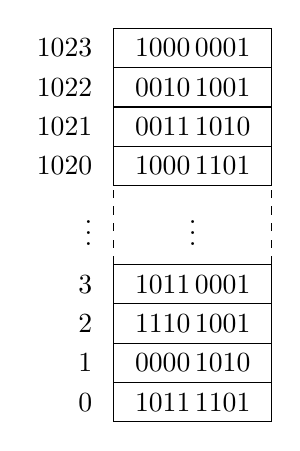
\begin{tikzpicture}
\pgfmathsetmacro{\kystep}{0.5}
\pgfmathsetmacro{\kxstep}{2}
\draw[](0,0)--++(0,4*\kystep) (0,6*\kystep)--++(0,4*\kystep)  (\kxstep,0)--++(0,4*\kystep)  (\kxstep,6*\kystep)--++(0,4*\kystep);
\draw[dashed](0,4*\kystep)--++(0,2*\kystep)  (\kxstep,4*\kystep)--++(0,2*\kystep);
\foreach \x in {0,1,2,3,4,6,7,8,9,10}{\draw(0,\x*\kystep)--++(\kxstep,0);}
\foreach \x/\a in {0/{1011\,1101},1/{0000\,1010},2/{1110\,1001},3/{1011\,0001}}{\draw(0.5*\kxstep,0.5*\kystep+\x*\kystep)node[]{$\a$};}
\foreach \x/\a in {6/{1000\,1101},7/{0011\,1010},8/{0010\,1001},9/{1000\,0001}}{\draw(0.5*\kxstep,0.5*\kystep+\x*\kystep)node[]{$\a$};}
\draw(0.5*\kxstep,5*\kystep)node[]{$\vdots$};
\draw(0,5*\kystep)node[left,xshift=-1ex]{$\vdots$};
\foreach \x/\a in {0/0,1/1,2/2,3/3,6/1020,7/1021,8/1022,9/1023}{\draw(0,0.5*\kystep+\x*\kystep)node[left,xshift=-1ex]{$\a$};}
\end{tikzpicture}
\end{subfigure}\hfill
\begin{subfigure}[b]{0.45\textwidth}
\centering
\begin{tikzpicture}
\pgfmathsetmacro{\kystep}{0.5}
\pgfmathsetmacro{\kxstep}{1.25}
\draw[](0,0)--++(0,4*\kystep)  (\kxstep,0)--++(0,4*\kystep);
\foreach \x in {0,1,2,3,4}{\draw(0,\x*\kystep)--++(\kxstep,0);}
\foreach \x/\a in {0/{0110},1/{0000},2/{1101},3/{1001}}{\draw(0.5*\kxstep,0.5*\kystep+\x*\kystep)node[]{$\a$};}
\foreach \x/\a in {0/00,1/01,2/10,3/11}{\draw(0,0.5*\kystep+\x*\kystep)node[left,xshift=-1ex]{$\a$};}
\draw(0,4*\kystep)node[above left,xshift=-1ex]{پتہ};
\draw(0.5*\kxstep,4*\kystep)node[above]{مواد};
\end{tikzpicture}
\end{subfigure}
\end{figure}
%========================
%fig 9.9
\begin{figure}
\centering
\begin{tikzpicture}[
 kmemUnit/.style={draw, minimum height=0.75cm, minimum width=0.75cm,thick,
 label={[anchor=west]center:اکائی},
 }]
\pgfmathsetmacro{\ksepX}{1.00}
\pgfmathsetmacro{\ksepY}{1.25}
\pgfmathsetmacro{\kpin}{0.5}
\pgfmathsetmacro{\kpinA}{0.3}
\pgfmathsetmacro{\kpsep}{0.50}
\pgfmathsetmacro{\kul}{0.50}
\pgfmathsetmacro{\kmv}{0.15}
\pgfmathsetmacro{\kxdim}{2*\kul+1*\kpsep}
\pgfmathsetmacro{\kydim}{2*\kul+3*\kpsep}
\draw(-0*\ksepX,0)node[or port,number inputs=4,scale=0.8,rotate=-90](u0){} (u0.out)node[below]{$D0$};
\draw(-1*\ksepX,0)node[or port,number inputs=4,scale=0.8,rotate=-90](u1){}(u1.out)node[below]{$D1$};
\draw(-2*\ksepX,0)node[or port,number inputs=4,scale=0.8,rotate=-90](u2){}(u2.out)node[below]{$D2$};
\draw(-3*\ksepX,0)node[or port,number inputs=4,scale=0.8,rotate=-90](u3){}(u3.out)node[below]{$D3$};
\draw(-4*\ksepX,0)node[or port,number inputs=4,scale=0.8,rotate=-90](u4){}(u4.out)node[below]{$D4$};
\draw(-5*\ksepX,0)node[or port,number inputs=4,scale=0.8,rotate=-90](u5){}(u5.out)node[below]{$D5$};
\draw(-6*\ksepX,0)node[or port,number inputs=4,scale=0.8,rotate=-90](u6){}(u6.out)node[below]{$D6$};
\draw(-7*\ksepX,0)node[or port,number inputs=4,scale=0.8,rotate=-90](u7){}(u7.out)node[below]{$D7$};
\draw[thick](-8*\ksepX,\ksepY) rectangle ++(-\kxdim,\kydim);
\draw(-8*\ksepX,\ksepY+\kul)node[left]{$y0$}coordinate(y0)--(y0 -| u0.in 1)--++(\kpinA,0)coordinate(kr)
node[right]{\RL{لفظ 0}};
\draw(-8*\ksepX,\ksepY+\kul+\kpsep)node[left]{$y1$}coordinate(y1)--(y1 -| kr);
\draw(-8*\ksepX,\ksepY+\kul+2*\kpsep)node[left]{$y2$}coordinate(y2)--(y2 -| kr);
\draw(-8*\ksepX,\ksepY+\kul+3*\kpsep)node[left]{$y3$}coordinate(y3)--(y3 -| kr)node[right]{\RL{لفظ 3}};
\draw(-8*\ksepX-\kxdim,\ksepY+\kul+2*\kpsep)node[right]{$a0$}--++(-\kpinA,0)node[left]{$A0$};
\draw(-8*\ksepX-\kxdim,\ksepY+\kul+3*\kpsep)node[right]{$a1$}--++(-\kpinA,0)node[left]{$A1$};
\draw(-8*\ksepX-\kxdim,\ksepY+\kul)node[right]{$e$}--++(-\kpinA,0)node[left]{مجاز};
\draw(-8*\ksepX,\ksepY)++(-0.5*\kxdim,\kydim)node[above]{\RL{شناخت کار}};
\draw(u0.in 1)--(u0.in 1 |- y0)   (u0.in 2)--(u0.in 2 |- y1)  (u0.in 3)--(u0.in 3 |- y2)  (u0.in 4)--(u0.in 4 |- y3);
\draw(u1.in 1)--(u1.in 1 |- y0)   (u1.in 2)--(u1.in 2 |- y1)  (u1.in 3)--(u1.in 3 |- y2)  (u1.in 4)--(u1.in 4 |- y3);
\draw(u2.in 1)--(u2.in 1 |- y0)   (u2.in 2)--(u2.in 2 |- y1)  (u2.in 3)--(u2.in 3 |- y2)  (u2.in 4)--(u2.in 4 |- y3);
\draw(u3.in 1)--(u3.in 1 |- y0)   (u3.in 2)--(u3.in 2 |- y1)  (u3.in 3)--(u3.in 3 |- y2)  (u3.in 4)--(u3.in 4 |- y3);
\draw(u4.in 1)--(u4.in 1 |- y0)   (u4.in 2)--(u4.in 2 |- y1)  (u4.in 3)--(u4.in 3 |- y2)  (u4.in 4)--(u4.in 4 |- y3);
\draw(u5.in 1)--(u5.in 1 |- y0)   (u5.in 2)--(u5.in 2 |- y1)  (u5.in 3)--(u5.in 3 |- y2)  (u5.in 4)--(u5.in 4 |- y3);
\draw(u6.in 1)--(u6.in 1 |- y0)   (u6.in 2)--(u6.in 2 |- y1)  (u6.in 3)--(u6.in 3 |- y2)  (u6.in 4)--(u6.in 4 |- y3);
\draw(u7.in 1)--(u7.in 1 |- y0)   (u7.in 2)--(u7.in 2 |- y1)  (u7.in 3)--(u7.in 3 |- y2)  (u7.in 4)--(u7.in 4 |- y3);
\end{tikzpicture}
\end{figure}
%======================
%fig 9.10
\begin{figure}
\centering
\begin{tikzpicture}[
 kmemUnit/.style={draw, minimum height=0.75cm, minimum width=0.75cm,thick,
 label={[anchor=west]center:اکائی},
 }]
\pgfmathsetmacro{\ksepX}{1.10}
\pgfmathsetmacro{\ksepY}{0.5}
\pgfmathsetmacro{\kpin}{0.5}
\pgfmathsetmacro{\kpinA}{0.3}
\pgfmathsetmacro{\kpsep}{0.50}
\pgfmathsetmacro{\kul}{0.50}
\pgfmathsetmacro{\kmv}{0.15}
\pgfmathsetmacro{\kxdim}{2*\kul+1*\kpsep}
\pgfmathsetmacro{\kydim}{2*\kul+3*\kpsep}
\kBusORdown[uu0]{-0*\ksepX}{0}
\kBusORdown[uu1]{-1*\ksepX}{0}
\kBusORdown[uu2]{-2*\ksepX}{0}
\kBusORdown[uu3]{-3*\ksepX}{0}
\kBusORdown[uu4]{-4*\ksepX}{0}
\kBusORdown[uu5]{-5*\ksepX}{0}
\kBusORdown[uu6]{-6*\ksepX}{0}
\kBusORdown[uu7]{-7*\ksepX}{0}
\draw(uu0out)--++(0,-\kpinA)node[below]{$D0$};
\draw(uu1out)--++(0,-\kpinA)node[below]{$D1$};
\draw(uu2out)--++(0,-\kpinA)node[below]{$D2$};
\draw(uu3out)--++(0,-\kpinA)node[below]{$D3$};
\draw(uu4out)--++(0,-\kpinA)node[below]{$D4$};
\draw(uu5out)--++(0,-\kpinA)node[below]{$D5$};
\draw(uu6out)--++(0,-\kpinA)node[below]{$D6$};
\draw(uu7out)--++(0,-\kpinA)node[below]{$D7$};
\draw[thick](-7*\ksepX-\kpin,\ksepY)coordinate(aa) rectangle ++(-\kxdim,\kydim)coordinate(tt);
\draw[thin](aa)++(0,\kul+0*\kpin)node[left]{$y0$}coordinate(bb)--(bb -| uu0in)--++(\kpinA,0)coordinate(krt)node[right]{};
\draw(aa)++(0,\kul+1*\kpin)node[left]{$y1$}coordinate(cc)--(cc -| krt);
\draw(aa)++(0,\kul+2*\kpin)node[left]{$y2$}coordinate(dd)--(dd -| krt);
\draw(aa)++(0,\kul+3*\kpin)node[left]{$y3$}coordinate(ee)--(ee -| krt);
\draw(aa)++(-0.5*\kxdim,\kydim)node[above]{\RL{شناخت کار}};
\draw(uu0in)--(uu0in |- tt);
\draw(uu1in)--(uu1in |- tt);
\draw(uu2in)--(uu2in |- tt);
\draw(uu3in)--(uu3in |- tt);
\draw(uu4in)--(uu4in |- tt);
\draw(uu5in)--(uu5in |- tt);
\draw(uu6in)--(uu6in |- tt);
\draw(uu7in)--(uu7in |- tt);
\draw(uu0in)++(-0.5*\kmv,\kpin)--++(\kmv,\kmv)node[right]{$4$}; 
\draw(uu1in)++(-0.5*\kmv,\kpin)--++(\kmv,\kmv)node[right]{$4$}; 
\draw(uu2in)++(-0.5*\kmv,\kpin)--++(\kmv,\kmv)node[right]{$4$}; 
\draw(uu3in)++(-0.5*\kmv,\kpin)--++(\kmv,\kmv)node[right]{$4$}; 
\draw(uu4in)++(-0.5*\kmv,\kpin)--++(\kmv,\kmv)node[right]{$4$}; 
\draw(uu5in)++(-0.5*\kmv,\kpin)--++(\kmv,\kmv)node[right]{$4$}; 
\draw(uu6in)++(-0.5*\kmv,\kpin)--++(\kmv,\kmv)node[right]{$4$}; 
\draw(uu7in)++(-0.5*\kmv,\kpin)--++(\kmv,\kmv)node[right]{$4$}; 
\draw[thin](aa)++(-\kxdim,\kul+0*\kpin)node[right]{$e$}--++(-\kpinA,0)node[left]{مجاز};
\draw[thin](aa)++(-\kxdim,\kul+2*\kpin)node[right]{$a0$}--++(-\kpinA,0)node[left]{$A0$};
\draw[thin](aa)++(-\kxdim,\kul+3*\kpin)node[right]{$a1$}--++(-\kpinA,0)node[left]{$A1$};
\end{tikzpicture}
\end{figure}
%=================

%fig 9.11
\begin{figure}
\centering
\begin{tikzpicture}[
 kmemUnit/.style={draw, minimum height=0.75cm, minimum width=0.75cm,thick,
 label={[anchor=west]center:اکائی},
 }]
\pgfmathsetmacro{\ksepX}{1.00}
\pgfmathsetmacro{\ksepY}{1.25}
\pgfmathsetmacro{\kpin}{0.5}
\pgfmathsetmacro{\kpinA}{0.3}
\pgfmathsetmacro{\kpsep}{0.50}
\pgfmathsetmacro{\kul}{0.50}
\pgfmathsetmacro{\kmv}{0.15}
\pgfmathsetmacro{\kxdim}{2*\kul+1*\kpsep}
\pgfmathsetmacro{\kydim}{2*\kul+3*\kpsep}
\draw(-0*\ksepX,0)node[or port,number inputs=4,scale=0.8,rotate=-90](u0){} (u0.out)node[below]{$D0$};
\draw(-1*\ksepX,0)node[or port,number inputs=4,scale=0.8,rotate=-90](u1){}(u1.out)node[below]{$D1$};
\draw(-2*\ksepX,0)node[or port,number inputs=4,scale=0.8,rotate=-90](u2){}(u2.out)node[below]{$D2$};
\draw(-3*\ksepX,0)node[or port,number inputs=4,scale=0.8,rotate=-90](u3){}(u3.out)node[below]{$D3$};
\draw(-4*\ksepX,0)node[or port,number inputs=4,scale=0.8,rotate=-90](u4){}(u4.out)node[below]{$D4$};
\draw(-5*\ksepX,0)node[or port,number inputs=4,scale=0.8,rotate=-90](u5){}(u5.out)node[below]{$D5$};
\draw(-6*\ksepX,0)node[or port,number inputs=4,scale=0.8,rotate=-90](u6){}(u6.out)node[below]{$D6$};
\draw(-7*\ksepX,0)node[or port,number inputs=4,scale=0.8,rotate=-90](u7){}(u7.out)node[below]{$D7$};
\draw[thick](-8*\ksepX,\ksepY) rectangle ++(-\kxdim,\kydim);
\draw(-8*\ksepX,\ksepY+\kul)node[left]{$y0$}coordinate(y0)--(y0 -| u0.in 1)--++(\kpinA,0)coordinate(kr)
node[right]{\RL{لفظ 0}};
\draw(-8*\ksepX,\ksepY+\kul+\kpsep)node[left]{$y1$}coordinate(y1)--(y1 -| kr);
\draw(-8*\ksepX,\ksepY+\kul+2*\kpsep)node[left]{$y2$}coordinate(y2)--(y2 -| kr);
\draw(-8*\ksepX,\ksepY+\kul+3*\kpsep)node[left]{$y3$}coordinate(y3)--(y3 -| kr)node[right]{\RL{لفظ 3}};
\draw(-8*\ksepX-\kxdim,\ksepY+\kul+2*\kpsep)node[right]{$a0$}--++(-\kpinA,0)node[left]{$A0$};
\draw(-8*\ksepX-\kxdim,\ksepY+\kul+3*\kpsep)node[right]{$a1$}--++(-\kpinA,0)node[left]{$A1$};
\draw(-8*\ksepX-\kxdim,\ksepY+\kul)node[right]{$e$}--++(-\kpinA,0)node[left]{مجاز};
\draw(-8*\ksepX,\ksepY)++(-0.5*\kxdim,\kydim)node[above]{\RL{شناخت کار}};
\draw(u0.in 1)--++(0,0.5*\kpin)   (u0.in 2)--(u0.in 2 |- y1)  (u0.in 3)--(u0.in 3 |- y2)  (u0.in 4)--(u0.in 4 |- y3);
\draw(u1.in 1)--++(0,0.5*\kpin)    (u1.in 2)--(u1.in 2 |- y1)  (u1.in 3)--(u1.in 3 |- y2)  (u1.in 4)--(u1.in 4 |- y3);
\draw(u2.in 1)--++(0,0.5*\kpin)    (u2.in 2)--(u2.in 2 |- y1)  (u2.in 3)--(u2.in 3 |- y2)  (u2.in 4)--(u2.in 4 |- y3);
\draw(u3.in 1)--++(0,0.5*\kpin)    (u3.in 2)--(u3.in 2 |- y1)  (u3.in 3)--(u3.in 3 |- y2)  (u3.in 4)--(u3.in 4 |- y3);
\draw(u4.in 1)--(u4.in 1 |- y0)   (u4.in 2)--(u4.in 2 |- y1)  (u4.in 3)--(u4.in 3 |- y2)  (u4.in 4)--(u4.in 4 |- y3);
\draw(u5.in 1)--(u5.in 1 |- y0)   (u5.in 2)--(u5.in 2 |- y1)  (u5.in 3)--(u5.in 3 |- y2)  (u5.in 4)--(u5.in 4 |- y3);
\draw(u6.in 1)--(u6.in 1 |- y0)   (u6.in 2)--(u6.in 2 |- y1)  (u6.in 3)--(u6.in 3 |- y2)  (u6.in 4)--(u6.in 4 |- y3);
\draw(u7.in 1)--(u7.in 1 |- y0)   (u7.in 2)--(u7.in 2 |- y1)  (u7.in 3)--(u7.in 3 |- y2)  (u7.in 4)--(u7.in 4 |- y3);
\end{tikzpicture}
\end{figure}
%======================
%fig 9.12
\begin{figure}
\centering
\begin{tikzpicture}[
 kmemUnit/.style={draw, minimum height=0.75cm, minimum width=0.75cm,thick,
 label={[anchor=west]center:اکائی},
 }]
\pgfmathsetmacro{\ksepX}{1.10}
\pgfmathsetmacro{\ksepY}{0.5}
\pgfmathsetmacro{\kpin}{0.5}
\pgfmathsetmacro{\kpinA}{0.3}
\pgfmathsetmacro{\kpsep}{0.50}
\pgfmathsetmacro{\kul}{0.50}
\pgfmathsetmacro{\kmv}{0.15}
\pgfmathsetmacro{\kxdim}{2*\kul+1*\kpsep}
\pgfmathsetmacro{\kydim}{2*\kul+3*\kpsep}
\kBusORdown[uu0]{-0*\ksepX}{0}
\kBusORdown[uu1]{-1*\ksepX}{0}
\kBusORdown[uu2]{-2*\ksepX}{0}
\kBusORdown[uu3]{-3*\ksepX}{0}
\kBusORdown[uu4]{-4*\ksepX}{0}
\kBusORdown[uu5]{-5*\ksepX}{0}
\kBusORdown[uu6]{-6*\ksepX}{0}
\kBusORdown[uu7]{-7*\ksepX}{0}
\draw(uu0out)--++(0,-\kpinA)node[below]{$D0$};
\draw(uu1out)--++(0,-\kpinA)node[below]{$D1$};
\draw(uu2out)--++(0,-\kpinA)node[below]{$D2$};
\draw(uu3out)--++(0,-\kpinA)node[below]{$D3$};
\draw(uu4out)--++(0,-\kpinA)node[below]{$D4$};
\draw(uu5out)--++(0,-\kpinA)node[below]{$D5$};
\draw(uu6out)--++(0,-\kpinA)node[below]{$D6$};
\draw(uu7out)--++(0,-\kpinA)node[below]{$D7$};
\draw[thick](-7*\ksepX-\kpin,\ksepY)coordinate(aa) rectangle ++(-\kxdim,\kydim)coordinate(tt);
\draw[thin](aa)++(0,\kul+0*\kpin)node[left]{$y0$}coordinate(bb)--(bb -| uu0in)--++(\kpinA,0)coordinate(krt)node[right]{};
\draw(aa)++(0,\kul+1*\kpin)node[left]{$y1$}coordinate(cc)--(cc -| krt);
\draw(aa)++(0,\kul+2*\kpin)node[left]{$y2$}coordinate(dd)--(dd -| krt);
\draw(aa)++(0,\kul+3*\kpin)node[left]{$y3$}coordinate(ee)--(ee -| krt);
\draw(aa)++(-0.5*\kxdim,\kydim)node[above]{\RL{شناخت کار}};
\draw(uu0in)--(uu0in |- tt);
\draw(uu1in)--(uu1in |- tt);
\draw(uu2in)--(uu2in |- tt);
\draw(uu3in)--(uu3in |- tt);
\draw(uu4in)--(uu4in |- tt);
\draw(uu5in)--(uu5in |- tt);
\draw(uu6in)--(uu6in |- tt);
\draw(uu7in)--(uu7in |- tt);
\draw(uu0in)++(-0.5*\kmv,\kpin)--++(\kmv,\kmv)node[right]{$4$}; 
\draw(uu1in)++(-0.5*\kmv,\kpin)--++(\kmv,\kmv)node[right]{$4$}; 
\draw(uu2in)++(-0.5*\kmv,\kpin)--++(\kmv,\kmv)node[right]{$4$}; 
\draw(uu3in)++(-0.5*\kmv,\kpin)--++(\kmv,\kmv)node[right]{$4$}; 
\draw(uu4in)++(-0.5*\kmv,\kpin)--++(\kmv,\kmv)node[right]{$4$}; 
\draw(uu5in)++(-0.5*\kmv,\kpin)--++(\kmv,\kmv)node[right]{$4$}; 
\draw(uu6in)++(-0.5*\kmv,\kpin)--++(\kmv,\kmv)node[right]{$4$}; 
\draw(uu7in)++(-0.5*\kmv,\kpin)--++(\kmv,\kmv)node[right]{$4$}; 
\draw[thin](aa)++(-\kxdim,\kul+0*\kpin)node[right]{$e$}--++(-\kpinA,0)node[left]{مجاز};
\draw[thin](aa)++(-\kxdim,\kul+2*\kpin)node[right]{$a0$}--++(-\kpinA,0)node[left]{$A0$};
\draw[thin](aa)++(-\kxdim,\kul+3*\kpin)node[right]{$a1$}--++(-\kpinA,0)node[left]{$A1$};
\path(uu0in)--(uu0in |- cc)coordinate(aaaa);
\draw(aaaa)++(-0.5*\kmv,-0.5*\kmv)--++(\kmv,\kmv)  (aaaa)++(-0.5*\kmv,0.5*\kmv)--++(\kmv,-\kmv);
\path(uu0in)--(uu0in |- dd)coordinate(aaaa);
\draw(aaaa)++(-0.5*\kmv,-0.5*\kmv)--++(\kmv,\kmv)  (aaaa)++(-0.5*\kmv,0.5*\kmv)--++(\kmv,-\kmv);
\path(uu1in)--(uu1in |- bb)coordinate(aaaa);
\draw(aaaa)++(-0.5*\kmv,-0.5*\kmv)--++(\kmv,\kmv)  (aaaa)++(-0.5*\kmv,0.5*\kmv)--++(\kmv,-\kmv);
\path(uu2in)--(uu2in |- cc)coordinate(aaaa);
\draw(aaaa)++(-0.5*\kmv,-0.5*\kmv)--++(\kmv,\kmv)  (aaaa)++(-0.5*\kmv,0.5*\kmv)--++(\kmv,-\kmv);
\path(uu2in)--(uu2in |- ee)coordinate(aaaa);
\draw(aaaa)++(-0.5*\kmv,-0.5*\kmv)--++(\kmv,\kmv)  (aaaa)++(-0.5*\kmv,0.5*\kmv)--++(\kmv,-\kmv);
\path(uu3in)--(uu3in |- dd)coordinate(aaaa);
\draw(aaaa)++(-0.5*\kmv,-0.5*\kmv)--++(\kmv,\kmv)  (aaaa)++(-0.5*\kmv,0.5*\kmv)--++(\kmv,-\kmv);
\path(uu3in)--(uu3in |- ee)coordinate(aaaa);
\draw(aaaa)++(-0.5*\kmv,-0.5*\kmv)--++(\kmv,\kmv)  (aaaa)++(-0.5*\kmv,0.5*\kmv)--++(\kmv,-\kmv);
\path(uu4in)--(uu4in |- bb)coordinate(aaaa);
\draw(aaaa)++(-0.5*\kmv,-0.5*\kmv)--++(\kmv,\kmv)  (aaaa)++(-0.5*\kmv,0.5*\kmv)--++(\kmv,-\kmv);
\path(uu5in)--(uu5in |- bb)coordinate(aaaa);
\draw(aaaa)++(-0.5*\kmv,-0.5*\kmv)--++(\kmv,\kmv)  (aaaa)++(-0.5*\kmv,0.5*\kmv)--++(\kmv,-\kmv);
\path(uu5in)--(uu5in |- cc)coordinate(aaaa);
\draw(aaaa)++(-0.5*\kmv,-0.5*\kmv)--++(\kmv,\kmv)  (aaaa)++(-0.5*\kmv,0.5*\kmv)--++(\kmv,-\kmv);
\path(uu5in)--(uu5in |- dd)coordinate(aaaa);
\draw(aaaa)++(-0.5*\kmv,-0.5*\kmv)--++(\kmv,\kmv)  (aaaa)++(-0.5*\kmv,0.5*\kmv)--++(\kmv,-\kmv);
\path(uu6in)--(uu6in |- cc)coordinate(aaaa);
\draw(aaaa)++(-0.5*\kmv,-0.5*\kmv)--++(\kmv,\kmv)  (aaaa)++(-0.5*\kmv,0.5*\kmv)--++(\kmv,-\kmv);
\path(uu6in)--(uu6in |- dd)coordinate(aaaa);
\draw(aaaa)++(-0.5*\kmv,-0.5*\kmv)--++(\kmv,\kmv)  (aaaa)++(-0.5*\kmv,0.5*\kmv)--++(\kmv,-\kmv);
\path(uu7in)--(uu7in |- bb)coordinate(aaaa);
\draw(aaaa)++(-0.5*\kmv,-0.5*\kmv)--++(\kmv,\kmv)  (aaaa)++(-0.5*\kmv,0.5*\kmv)--++(\kmv,-\kmv);
\path(uu7in)--(uu7in |- ee)coordinate(aaaa);
\draw(aaaa)++(-0.5*\kmv,-0.5*\kmv)--++(\kmv,\kmv)  (aaaa)++(-0.5*\kmv,0.5*\kmv)--++(\kmv,-\kmv);
\end{tikzpicture}
\end{figure}
%=================
%fig 9.13
\begin{figure}
\centering
\begin{subfigure}{1\textwidth}
\centering
\begin{tikzpicture}
\pgfmathsetmacro{\ksepX}{1.10}
\pgfmathsetmacro{\ksepY}{4}
\pgfmathsetmacro{\kpin}{0.5}
\pgfmathsetmacro{\kpinA}{0.3}
\pgfmathsetmacro{\kpsep}{0.50}
\pgfmathsetmacro{\kul}{0.50}
\pgfmathsetmacro{\kmv}{0.15}
\pgfmathsetmacro{\kxdim}{2*\kul+2*\kpsep}
\pgfmathsetmacro{\kydim}{2*\kul+4*\kpsep}
\draw[thick](0,0) rectangle++(\kxdim,\kydim);
\draw[thick](0,\ksepY) rectangle++(\kxdim,\kydim);
\draw(0.5*\kxdim,\kydim)node[above]{\text{\RL{\عددی{4\times 4}  حافظہ 0}}};
\draw(0.5*\kxdim,\ksepY+\kydim)node[above]{\text{\RL{\عددی{4\times 4}  حافظہ 1}}};
\draw(0,\ksepY)++(\kxdim,\kul+1*\kpsep)coordinate(aa)node[left]{$I\!/\!O 0$}--++(5*\kpin,0)node[right]{$D0$};
\draw(0,\ksepY)++(\kxdim,\kul+2*\kpsep)coordinate(bb)node[left]{$I\!/\!O 1$}--++(5*\kpin,0)node[right]{$D1$};
\draw(0,\ksepY)++(\kxdim,\kul+3*\kpsep)coordinate(cc)node[left]{$I\!/\!O 2$}--++(5*\kpin,0)node[right]{$D2$};
\draw(0,\ksepY)++(\kxdim,\kul+4*\kpsep)coordinate(dd)node[left]{$I\!/\!O 3$}--++(5*\kpin,0)node[right]{$D3$};
\draw(\kxdim,\kul+4*\kpsep)node[left]{$I\!/\!O 3$}--++(\kpin,0)coordinate(ee)--(ee |- dd);
\draw(\kxdim,\kul+3*\kpsep)node[left]{$I\!/\!O 2$}--++(2*\kpin,0)coordinate(ff)--(ff |- cc);
\draw(\kxdim,\kul+2*\kpsep)node[left]{$I\!/\!O 1$}--++(3*\kpin,0)coordinate(gg)--(gg |- bb);
\draw(\kxdim,\kul+1*\kpsep)node[left]{$I\!/\!O 0$}--++(4*\kpin,0)coordinate(hh)--(hh |- aa);
\draw(0,\ksepY+\kul)node[right]{$\overline{\text{\RL{بیدار1}}}$}--++(-4*\kpin,0)node[not port,scale=1,anchor=out](u0){};
\draw(0,\ksepY+\kul)++(-0.05,0)node[ocirc]{};
\draw(u0.in)--++(-\kpin,0)coordinate(klft)node[left]{$A2$};
\draw(0,\kul)node[right]{$\overline{\text{\RL{بیدار0}}}$}-|(u0.in);
\draw(0,\kul)++(-0.05,0)node[ocirc]{};
\draw(0,\kul+\kpin)coordinate(rd)--(rd -| klft)node[left]{$\overline{\text{لکھ}}/\text{پرھ}$};
\draw(0,\kul+\kpin)node[right]{$\overline{\text{لکھ}}$}++(-0.05,0)node[ocirc]{};
\draw(0,\kul+3*\kpin)node[right]{$a0$}coordinate(ka0)--(ka0 -| klft)node[left]{$A0$};
\draw(0,\kul+4*\kpin)node[right]{$a1$}coordinate(ka1)--(ka1 -| klft)node[left]{$A1$};
\draw(0,\ksepY+\kul+1*\kpin)node[right]{$\overline{\text{لکھ}}$}--++(-\kpin,0)coordinate(kka)--(kka |- rd);
\draw(0,\ksepY+\kul+1*\kpin)++(-0.05,0)node[ocirc]{};
\draw(0,\ksepY+\kul+3*\kpin)node[right]{$a0$}--++(-2*\kpin,0)coordinate(kka0)--(kka0|- ka0);
\draw(0,\ksepY+\kul+4*\kpin)node[right]{$a1$}--++(-3*\kpin,0)coordinate(kka1)--(kka1|- ka1);
\end{tikzpicture}
\caption{}
\end{subfigure}
\begin{subfigure}{1\textwidth}
\centering
\begin{tikzpicture}
\pgfmathsetmacro{\ksepX}{1.10}
\pgfmathsetmacro{\ksepY}{4}
\pgfmathsetmacro{\kpin}{0.5}
\pgfmathsetmacro{\kpinA}{0.3}
\pgfmathsetmacro{\kpsep}{0.50}
\pgfmathsetmacro{\kul}{0.50}
\pgfmathsetmacro{\kmv}{0.15}
\pgfmathsetmacro{\kxdim}{2*\kul+2*\kpsep}
\pgfmathsetmacro{\kydim}{2*\kul+4*\kpsep}
\draw[thick](0,0) rectangle++(\kxdim,\kydim);
\draw(0.5*\kxdim,\kydim)node[above]{\text{\RL{\عددی{8\times 4}  حافظہ}}};
\foreach \x/\a/\b in {0/a0/A0,1/a1/A1,2/a2/A2}{\draw(0,\kul+2*\kpsep+\x*\kpsep)node[right]{$\a$}--++(-\kpin,0)node[left]{$\b$};}
\foreach \x/\a/\b in {0/{I/O0}/D0,1/{I/O1}/D1,2/{I/O2}/D2,3/{I/O3}/D3}{\draw(\kxdim,\kul+\kpin+\x*\kpsep)node[left]{$\a$}--++(\kpin,0)node[right]{$\b$};}
\draw(0,\kul)node[right]{$\overline{\text{لکھ}}$}--++(-\kpin,0)node[left]{$\overline{\text{لکھ}}/\text{پڑھ}$};
\draw(0,\kul)++(-0.05,0)node[ocirc]{};
\end{tikzpicture}
\caption{}
\end{subfigure}
\end{figure}
%=======================
%fig 9.14
\begin{figure}
\centering
\begin{subfigure}{1\textwidth}
\centering
\begin{tikzpicture}
\pgfmathsetmacro{\kystep}{0.5}
\pgfmathsetmacro{\kxstep}{1}
\foreach \x/\a in {0/1,1/1,2/1,3/1,4/0,5/0,6/0,7/0,8/{A2}}{\draw(0,\x*\kystep)node[]{$\a$};}
\foreach \x/\a in {0/1,1/1,2/0,3/0,4/1,5/1,6/0,7/0,8/{A1}}{\draw(\kxstep,\x*\kystep)node[]{$\a$};}
\foreach \x/\a in {0/1,1/0,2/1,3/0,4/1,5/0,6/1,7/0,8/{A0}}{\draw(2*\kxstep,\x*\kystep)node[]{$\a$};}
\draw(-0.5*\kxstep,7.5*\kystep)--++(3*\kxstep,0);
\draw[dashed](0,5.5*\kystep) circle (0.5 and 1.9*\kystep);
\draw[](-0.5,5.5*\kystep) to [out=180,in=-45]++(-2,0.25)node[above]{\RL{حافظہ \عددی{0} بیدار ہے}};
\draw[dashed](0,1.5*\kystep) circle (0.5 and 1.9*\kystep);
\draw[](-0.5,1.5*\kystep) to [out=180,in=45]++(-2,-0.25)node[below]{\RL{حافظہ \عددی{1} بیدار ہے}};
\draw[dashed](0.75*\kxstep,6.5*\kystep) rectangle ++(1.5*\kxstep,0.9*\kystep);
\draw[] (0.75*\kxstep,6.5*\kystep) ++(1.5*\kxstep,0.45*\kystep) to [out=0,in=-150]++(2,0.25)node[right]{\RL{حافظہ \عددی{0} کا مقام \عددی{0}}};
\draw[dashed](0.75*\kxstep,2.5*\kystep) rectangle ++(1.5*\kxstep,0.9*\kystep);
\draw[] (0.75*\kxstep,2.5*\kystep) ++(1.5*\kxstep,0.45*\kystep) to [out=0,in=-150]++(2,0.25)node[right]{\RL{حافظہ \عددی{1} کا مقام \عددی{0}}};
\end{tikzpicture}
\caption{}
\end{subfigure}
\begin{subfigure}{1\textwidth}
\centering
\begin{tikzpicture}
\pgfmathsetmacro{\kystep}{0.5}
\pgfmathsetmacro{\kxstep}{1.25}
\pgfmathsetmacro{\ksepX}{4}
\pgfmathsetmacro{\ksepY}{0.25}
\draw[](0,0)--++(0,8*\kystep)  (\kxstep,0)--++(0,8*\kystep);
\foreach \x in {0,1,...,8}{\draw(0,\x*\kystep)--++(\kxstep,0);}
\foreach \x in {0,1,...,7}{\draw(0.5*\kxstep,0.5*\kystep+\x*\kystep)node[]{\RL{مقام \, \x}};}
\draw(0.5*\kxstep,0)node[below]{$8\times 4$};
\draw[](-\ksepX,-\ksepY)--++(0,4*\kystep)  (-\ksepX+\kxstep,-\ksepY)--++(0,4*\kystep);
\foreach \x in {0,1,...,4}{\draw(-\ksepX,-\ksepY+\x*\kystep)--++(\kxstep,0);}
\foreach \x in {0,1,...,3}{\draw(-\ksepX+0.5*\kxstep,-\ksepY+0.5*\kystep+\x*\kystep)node[]{\RL{مقام \, \x}};}
\draw[](-\ksepX,\ksepY+4*\kystep)--++(0,4*\kystep)  (-\ksepX+\kxstep,\ksepY+4*\kystep)--++(0,4*\kystep);
\foreach \x in {0,1,...,4}{\draw(-\ksepX,\ksepY+\x*\kystep+4*\kystep)--++(\kxstep,0);}
\foreach \x in {0,1,...,3}{\draw(-\ksepX+0.5*\kxstep,\ksepY+0.5*\kystep+\x*\kystep+4*\kystep)node[]{\RL{مقام \, \x}};}
\draw[decorate,decoration={brace,amplitude=10pt, raise=2pt}](0,0.1)--++(0,4*\kystep-0.2);
\draw[decorate,decoration={brace,amplitude=10pt, raise=2pt}](0,4*\kystep+0.1)--(0,8*\kystep-0.1);
\draw[decorate,decoration={brace,amplitude=10pt, raise=2pt,mirror}](-\ksepX+\kxstep,-\ksepY+0.1)--++(0,4*\kystep-0.2);
\draw[decorate,decoration={brace,amplitude=10pt, raise=2pt,mirror}](-\ksepX+\kxstep,4*\kystep+\ksepY+0.1)--++(0,4*\kystep-0.2);
\draw[-stealth] (-\ksepX+\kxstep+0.5,-\ksepY+2*\kystep) to [out=0,in=180] (-0.5,2*\kystep);
\draw[-stealth] (-\ksepX+\kxstep+0.5,\ksepY+6*\kystep) to [out=0,in=180] (-0.5,6*\kystep);
\draw(-\ksepX,-\ksepY+2*\kystep)node[left]{\RL{\عددی{4\times 4} حافظہ 0}};
\draw(-\ksepX,\ksepY+6*\kystep)node[left]{\RL{\عددی{4\times 4} حافظہ 1}};
\end{tikzpicture}
\caption{}
\end{subfigure}
\end{figure}
%===========================
%fig 9.15
\begin{figure}
\centering
\begin{tikzpicture}
\pgfmathsetmacro{\kpin}{0.5}
\pgfmathsetmacro{\kpinA}{0.3}
\pgfmathsetmacro{\kpsep}{0.50}
\pgfmathsetmacro{\kul}{0.50}
\pgfmathsetmacro{\kmv}{0.15}
\pgfmathsetmacro{\kxdim}{2*\kul+2*\kpsep}
\pgfmathsetmacro{\kydim}{2*\kul+7*\kpsep}
\pgfmathsetmacro{\ksepX}{1.10}
\pgfmathsetmacro{\ksepY}{\kydim+0.75}
\draw[thick](0,0) rectangle++(\kxdim,\kydim);
\draw[thick](0,\ksepY) rectangle++(\kxdim,\kydim);
\draw[thick](0,2*\ksepY) rectangle++(\kxdim,\kydim);
\draw(0.5*\kxdim,\kydim)node[above]{\text{\RL{حافظہ 0}}};
\draw(0.5*\kxdim,\ksepY+\kydim)node[above]{\text{\RL{حافظہ 1}}};
\draw(0.5*\kxdim,2*\ksepY+\kydim)node[above]{\text{\RL{حافظہ 2}}};
\foreach \x in {0,1,...,7}{\draw(\kxdim,2*\ksepY+\kul+\x*\kpsep)node[left]{$I\!/\!O_\x$}--++(\kpin+3.5*\kpin+\kpin,0)node[right]{$D_\x$};}
\foreach \x in {0,1,...,7}{\draw(\kxdim,\kul+\x*\kpsep)node[left]{$I\!/\!O_\x$}--++(\kpin+3.5*\kpin-\x*0.5*\kpin,0)--++(0,2*\ksepY);}
\foreach \x in {0,1,...,7}{\draw(\kxdim,\ksepY+\kul+\x*\kpsep)node[left]{$I\!/\!O_\x$}--++(\kpin+3.5*\kpin-\x*0.5*\kpin,0);}
\foreach \x in {0,1,2,3}{\draw(0,2*\ksepY+\kul+3*\kpsep+\x*\kpsep)node[right]{$A_\x$}--++(-3*\kxdim-\kpin,0)node[left]{$A_\x$};}
\foreach \x in {0,1,2,3}{\draw(0,0*\ksepY+\kul+3*\kpsep+\x*\kpsep)node[right]{$A_\x$}--++(-\kpin-2*\kpin+0.5*\x*\kpin,0)--++(0,2*\ksepY);}
\foreach \x in {0,1,2,3}{\draw(0,1*\ksepY+\kul+3*\kpsep+\x*\kpsep)node[right]{$A_\x$}--++(-\kpin-2*\kpin+0.5*\x*\kpin,0);}
\draw[thick](-3*\kxdim,2*\ksepY+\kydim-1*\kpsep) rectangle ++(\kxdim,2*\kul+3*\kpsep)coordinate(kDecoder);
\draw(kDecoder)++(-0.5*\kxdim,0)node[above]{\RL{شناخت کار}};
\foreach \x/\a in {0/4,1/5}{\draw(-3*\kxdim,2*\ksepY+\kydim-1*\kpsep+\kul+\kpsep+\x*\kpsep)node[right]{$a_\x$}--++(-\kpin,0)node[left]{$A_\a$};}
\draw(-3*\kxdim+\kxdim,2*\ksepY+\kydim-1*\kpsep+\kul+0*\kpsep)node[left]{$\overline{y_0}$}--++(\kpin,0)|-(0,\kul)node[right]{$\overline{\text{\RL{بیدار0}}}$}; 
\draw(-3*\kxdim+\kxdim,2*\ksepY+\kydim-1*\kpsep+\kul+1*\kpsep)node[left]{$\overline{y_1}$}--++(\kpin+0.5*\kpin,0)|-(0,\ksepY+\kul)node[right]{$\overline{\text{\RL{بیدار1}}}$}; 
\draw(-3*\kxdim+\kxdim,2*\ksepY+\kydim-1*\kpsep+\kul+3*\kpsep)node[left]{$\overline{y_3}$}--++(\kpin+\kpin,0)|-(0,2*\ksepY+\kul)node[right]{$\overline{\text{\RL{بیدار3}}}$}; 
\draw(-3*\kxdim+\kxdim,2*\ksepY+\kydim-1*\kpsep+\kul+2*\kpsep)node[left]{$\overline{y_2}$}--++(0.5*\kpin,0);
\foreach \x in {0,1,2,3}{\draw(-3*\kxdim+\kxdim,2*\ksepY+\kydim-1*\kpsep+\kul+\x*\kpsep)++(0.05,0)node[ocirc]{};}
\draw(0,2*\ksepY+\kul+1*\kpsep)node[right]{$\overline{\text{لکھ}}$}--++(-3*\kxdim-\kpin,0)coordinate[pos=0.4](rdWr)node[left]{$\overline{\text{لکھ}}/\text{پڑھ}$};
\draw(rdWr)|-(0,\kul+\kpsep)node[right]{$\overline{\text{لکھ}}$};
\draw(0,\ksepY+\kul+\kpsep)coordinate(kkL)node[right]{$\overline{\text{لکھ}}$}--(kkL -| rdWr);
\foreach \x in {0,1}{\draw(0,\kul+\x*\kpsep)++(-0.05,0)node[ocirc]{};}
\foreach \x in {0,1}{\draw(0,\ksepY+\kul+\x*\kpsep)++(-0.05,0)node[ocirc]{};}
\foreach \x in {0,1}{\draw(0,2*\ksepY+\kul+\x*\kpsep)++(-0.05,0)node[ocirc]{};}
\end{tikzpicture}
\end{figure}
%========================
% fig 9-15a
\begin{figure}
\centering
\begin{tikzpicture}
\pgfmathsetmacro{\kystep}{0.15}
\pgfmathsetmacro{\kxstep}{1.25}
\pgfmathsetmacro{\ksepX}{4}
\pgfmathsetmacro{\ksepY}{0.25}
\draw[](0,0)--++(0,32*\kystep)  (\kxstep,0)--++(0,32*\kystep);
\foreach \x in {0,1,...,32}{\draw(0,\x*\kystep)--++(\kxstep,0);}
\draw[](0,48*\kystep)--++(0,16*\kystep)  (\kxstep,48*\kystep)--++(0,16*\kystep);
\foreach \x in {0,1,...,16}{\draw(0,48*\kystep+\x*\kystep)--++(\kxstep,0);}
\draw(0,32*\kystep)--++(0,16*\kystep)  (\kxstep,32*\kystep)--++(0,16*\kystep);
\draw[](-\ksepX,0)--++(0,16*\kystep)  (-\ksepX+\kxstep,0)--++(0,16*\kystep);
\foreach \x in {0,1,...,16}{\draw(-\ksepX,\x*\kystep)--++(\kxstep,0);}
\draw(-\ksepX,8*\kystep)node[left]{\RL{حافظہ 0}};
\draw[](-\ksepX,\ksepY+16*\kystep)--++(0,16*\kystep)  (-\ksepX+\kxstep,\ksepY+16*\kystep)--++(0,16*\kystep);
\foreach \x in {0,1,...,16}{\draw(-\ksepX,\ksepY+16*\kystep+\x*\kystep)--++(\kxstep,0);}
\draw(-\ksepX,\ksepY+16*\kystep+8*\kystep)node[left]{\RL{حافظہ 1 }};
\draw[](-\ksepX,2*\ksepY+32*\kystep)--++(0,16*\kystep)  (-\ksepX+\kxstep,2*\ksepY+32*\kystep)--++(0,16*\kystep);
\foreach \x in {0,1,...,16}{\draw(-\ksepX,2*\ksepY+32*\kystep+\x*\kystep)--++(\kxstep,0);}
\draw(-\ksepX,2*\ksepY+32*\kystep+8*\kystep)node[left]{\RL{حافظہ 2 }};
\draw[decorate,decoration={brace,amplitude=10pt, raise=2pt}](0,0)--++(0,16*\kystep);
\draw[decorate,decoration={brace,amplitude=10pt, raise=2pt}](0,16*\kystep)--++(0,16*\kystep);
\draw[decorate,decoration={brace,amplitude=10pt, raise=2pt}](0,48*\kystep)--++(0,16*\kystep);
\draw(-0.50,8*\kystep) to [out=170,in=20] (-\ksepX+\kxstep+0.2,10*\kystep);
\draw(-0.50,24*\kystep) to [out=170,in=20] (-\ksepX+\kxstep+0.2,\ksepY+26*\kystep);
\draw(-0.50,56*\kystep) to [out=-170,in=45] (-\ksepX+\kxstep+0.2,\ksepY+42*\kystep);
\draw(0.5*\kxstep,40*\kystep)node[rotate=90,above]{\RL{غیر مستعمل}}node[rotate=90,below]{\RL{مقامات}};
\end{tikzpicture}
\caption{}
\end{figure}
%============================
%fig 9.16
\begin{figure}
\centering
\begin{subfigure}{0.55\textwidth}
\centering
\begin{tikzpicture}
\pgfmathsetmacro{\kpin}{0.5}
\pgfmathsetmacro{\kpinA}{0.3}
\pgfmathsetmacro{\kpsep}{0.50}
\pgfmathsetmacro{\kul}{0.50}
\pgfmathsetmacro{\kmv}{0.15}
\pgfmathsetmacro{\kxdim}{2*\kul+2*\kpsep}
\pgfmathsetmacro{\kydim}{2*\kul+4*\kpsep}
\pgfmathsetmacro{\ksepX}{1.10}
\pgfmathsetmacro{\ksepY}{\kydim+0.75}
\draw[thick](0,0) rectangle++(\kxdim,\kydim);
\draw[thick](0,\ksepY) rectangle++(\kxdim,\kydim);
\draw(0.5*\kxdim,\kydim)node[above]{\text{\RL{حافظہ 0}}};
\draw(0.5*\kxdim,\ksepY+\kydim)node[above]{\text{\RL{حافظہ 1}}};
\foreach \x/\a in {0/4,1/5,2/6,3/7}{\draw(\kxdim,1*\ksepY+\kul+\kpin+\x*\kpsep)node[left]{$I\!/\!O_\x$}--++(\kpin,0)node[right]{$D_\a$};}
\foreach \x in {0,1,2,3}{\draw(\kxdim,0*\ksepY+\kul+\kpin+\x*\kpsep)node[left]{$I\!/\!O_\x$}--++(\kpin,0)node[right]{$D_\x$};}
\foreach \x in {0,1}{\draw(0,\kul+3*\kpin+\x*\kpin)node[right]{$A_\x$}--++(-4*\kpin,0)node[left]{$A_\x$};}
\draw(0,\kul)node[right]{$\overline{\text{\RL{بیدار 0}}}$}--++( -4*\kpin,0)node[left]{$\overline{\text{\RL{بیدار}}}$};
\draw(0,\kul+\kpin)node[right]{$\overline{\text{\RL{لکھ}}}$}--++( -4*\kpin,0)node[left]{$\overline{\text{\RL{لکھ}}}/\text{پڑھ}$};
\draw(0,\ksepY+\kul+3*\kpin)node[right]{$A_0$}--++(-2*\kpin,0)coordinate(aa)--(aa|- 0,\kul+3*\kpin);
\draw(0,\ksepY+\kul+4*\kpin)node[right]{$A_1$}--++(-2.5*\kpin,0)coordinate(aa)--(aa|- 0,\kul+4*\kpin);
\draw(0,\ksepY+\kul)node[right]{$\overline{\text{\RL{بیدار 1}}}$}--++(-1*\kpin,0)coordinate(aa)--(aa|- 0,\kul);
\draw(0,\ksepY+\kul+\kpin)node[right]{$\overline{\text{\RL{لکھ}}}$}--++(-1.5*\kpin,0)coordinate(aa)--(aa|- 0,\kul+\kpin);
\foreach \x in {0,1}{\draw(0,\kul+\x*\kpin)++(-0.05,0)node[ocirc]{}  (0,\ksepY+\kul+\x*\kpin)++(-0.05,0)node[ocirc]{};}
\end{tikzpicture}
\caption{}
\end{subfigure}\hfill
\begin{subfigure}{0.35\textwidth}
\centering
\begin{tikzpicture}
\pgfmathsetmacro{\kpin}{0.5}
\pgfmathsetmacro{\kpinA}{0.3}
\pgfmathsetmacro{\kpsep}{0.50}
\pgfmathsetmacro{\kul}{0.50}
\pgfmathsetmacro{\kmv}{0.15}
\pgfmathsetmacro{\kxdim}{2*\kul+2*\kpsep}
\pgfmathsetmacro{\kydim}{2*\kul+7*\kpsep}
\pgfmathsetmacro{\ksepX}{1.10}
\pgfmathsetmacro{\ksepY}{\kydim+0.75}
\draw[thick](0,0) rectangle++(\kxdim,\kydim);
\draw(0.5*\kxdim,\kydim)node[above]{حافظہ}node[above,yshift=0.5cm]{$4\times 8$};
\foreach \x in {0,1,...,7}{\draw(\kxdim,\kul+\x*\kpsep)node[left]{$I\!/\!O_\x$}--++(\kpin,0)node[right]{$D_\x$};}
\foreach \x in {0,1}{\draw(0,\kul+5*\kpin+\x*\kpsep)node[right]{$A_\x$}--++(-\kpin,0)node[left]{$A_\x$};}
\draw(0,\kul)node[right]{$\overline{\text{بیدار}}$}--++(-\kpin,0)node[left]{$\overline{\text{بیدار}}$};
\draw(0,\kul+\kpin)node[right]{$\overline{\text{لکھ}}$}--++(-\kpin,0)node[left]{$\overline{\text{لکھ}}/{\text{پڑھ}}$};
\draw(0,\kul)++(-0.05,0)node[ocirc]{};
\draw(0,\kul+\kpin)++(-0.05,0)node[ocirc]{};
\end{tikzpicture}
\caption{}
\end{subfigure}
\end{figure}
%========================
\begin{figure}
\centering
\begin{subfigure}{1\textwidth}
\centering
\begin{otherlanguage}{english}
 \begin{tikztimingtable}[%
timing/.style={x=2ex,y=3ex},
timing/rowdist=5ex,
every node/.style={inner sep=0,outer sep=0},
timing/c/arrow tip=latex, %and this set the style
timing/c/rising arrows,
timing/slope=0.3, %0.1 is good
timing/dslope=0.3,
thick,
]
%\tikztimingmetachar{R}{[|/utils/exec=\setcounter{new}{0}|]}
%\usetikztiminglibrary[new={char=Q,reset char=R}]{counters}
%[timing/counter/new={char=c, base=2,digits=3,max value=7, wraps ,text style={font=\normalsize}}] 12{2c} \\ 
%$C$& H22{C}\\
$\texturdu{\RL{پتہ}}$&3D{} 20D{[scale=1.5]\texturdu{\RL{درست پتہ}}} 3D{}\\
$\overline{\texturdu{\RL{بیدار}}}$&3H 0.2h 20L 3H\\
$\overline{\texturdu{\RL{لکھ}}}/\texturdu{\RL{پڑھ}}$&5H16L5H\\
$\texturdu{\RL{مداخل مواد}}$&6.5D{}18D{[scale=1.5]\texturdu{\RL{درست مواد}}}1.5D\\ 
\extracode
%\begin{pgfonlayer}{background}
%\begin{scope}[semitransparent ,dashed]
%%\vertlines[darkgray,dotted]{3.6,7.5,11.5,15.5,19.5,23.5,27.5}
%\foreach \n in {1,3,...,11} \draw(4*\n ex-2ex,-4ex+1.25ex)node[]{$0$};
%\foreach \n in {2,4,...,12} \draw(4*\n ex-2ex,-4ex+1.25ex)node[]{$1$};
%\foreach \n in {1,2,5,6,9,10} \draw(4*\n ex-2ex,-12 ex+1.25ex)node[]{$0$};
%\foreach \n in {3,4,7,8,11,12} \draw(4*\n ex-2ex,-12 ex+1.25ex)node[]{$1$};
%\foreach \n in {1,2,3,4,9,10,11,12} \draw(4*\n ex-2ex,-20 ex+1.25ex)node[]{$0$};
%\foreach \n in {5,6,7,8} \draw(4*\n ex-2ex,-20 ex+1.25ex)node[]{$1$};
%\draw(4*4 ex-2ex,-12 ex+1.25ex) circle (0.25cm and 1.75cm);
%\draw(4*4 ex-2ex,-7*\rowdist+1.25ex) circle (0.25cm and 0.5cm);
%%\foreach \n in {1}\draw(B\n.south)--(F\n.north);
%%\foreach \n in {1}\draw(C\n.south)--(G\n.north);
%\end{scope}
%\end{pgfonlayer}
\end{tikztimingtable}
\end{otherlanguage}
\caption{حافظہ میں مواد لکھنے کا عمل}
\end{subfigure}
\begin{subfigure}{1\textwidth}
\centering
\begin{otherlanguage}{english}
 \begin{tikztimingtable}[%
timing/.style={x=2ex,y=3ex},
timing/rowdist=5ex,
every node/.style={inner sep=0,outer sep=0},
timing/c/arrow tip=latex, %and this set the style
timing/c/rising arrows,
timing/slope=0.3, %0.1 is good
timing/dslope=0.3,
thick,
]
%\tikztimingmetachar{R}{[|/utils/exec=\setcounter{new}{0}|]}
%\usetikztiminglibrary[new={char=Q,reset char=R}]{counters}
%[timing/counter/new={char=c, base=2,digits=3,max value=7, wraps ,text style={font=\normalsize}}] 12{2c} \\ 
%$C$& H22{C}\\
$\texturdu{\RL{پتہ}}$&3D{} 20D{[scale=1.5]\texturdu{\RL{درست پتہ}}} 3D{}\\
$\overline{\texturdu{\RL{بیدار}}}$&3H 0.2h 20L 3H\\
$\overline{\texturdu{\RL{لکھ}}}/\texturdu{\RL{پڑھ}}$&5H16H5H\\
$\texturdu{\RL{مخارج  مواد}}$&16.5D{}8D{[scale=1.5]\texturdu{\RL{درست مواد}}}1.5D\\ 
\extracode
\begin{pgfonlayer}{background}
%\begin{scope}[semitransparent ,dashed]
\draw[dashed](6.5 ex,-1*\rowdist)--++(0,-3*\rowdist)coordinate(aa);
\draw[dashed](2*16.5 ex+0.25 ex,-3*\rowdist)--++(0,-1*\rowdist)coordinate(bb);
\draw[stealth-stealth]($(aa)+(0,1 ex)$)--($(bb)+(0,1 ex)$)node[pos=0.5,fill=white]{\texturdu{\RL{دورانیہ رسائی}}};
%\vertlines[darkgray,dotted]{3.6,7.5,11.5,15.5,19.5,23.5,27.5}
%\foreach \n in {1,3,...,11} \draw(4*\n ex-2ex,-4ex+1.25ex)node[]{$0$};
%\foreach \n in {2,4,...,12} \draw(4*\n ex-2ex,-4ex+1.25ex)node[]{$1$};
%\foreach \n in {1,2,5,6,9,10} \draw(4*\n ex-2ex,-12 ex+1.25ex)node[]{$0$};
%\foreach \n in {3,4,7,8,11,12} \draw(4*\n ex-2ex,-12 ex+1.25ex)node[]{$1$};
%\foreach \n in {1,2,3,4,9,10,11,12} \draw(4*\n ex-2ex,-20 ex+1.25ex)node[]{$0$};
%\foreach \n in {5,6,7,8} \draw(4*\n ex-2ex,-20 ex+1.25ex)node[]{$1$};
%\draw(4*4 ex-2ex,-12 ex+1.25ex) circle (0.25cm and 1.75cm);
%\draw(4*4 ex-2ex,-7*\rowdist+1.25ex) circle (0.25cm and 0.5cm);
%%\foreach \n in {1}\draw(B\n.south)--(F\n.north);
%%\foreach \n in {1}\draw(C\n.south)--(G\n.north);
%\end{scope}
\end{pgfonlayer}
\end{tikztimingtable}
\end{otherlanguage}
\caption{حافظہ سے مواد پڑھنے کا عمل}
\end{subfigure}
\end{figure}
